\documentclass[../main-v2-manifolds.tex]{subfiles}


\begin{document}
%%%%%%%%%
%%%%%%%%%
%%%%%%%%%
\makeatletter
\newcommand*{\addFileDependency}[1]{% argument=file name and extension
\typeout{(#1)}% latexmk will find this if $recorder=0
% however, in that case, it will ignore #1 if it is a .aux or 
% .pdf file etc and it exists! If it doesn't exist, it will appear 
% in the list of dependents regardless)
%
% Write the following if you want it to appear in \listfiles 
% --- although not really necessary and latexmk doesn't use this
%
\@addtofilelist{#1}
%
% latexmk will find this message if #1 doesn't exist (yet)
\IfFileExists{#1}{}{\typeout{No file #1.}}
}\makeatother

\newcommand*{\myexternaldocument}[1]{%
\externaldocument{#1}%
\addFileDependency{#1.tex}%
\addFileDependency{#1.aux}%
}
%------------End of helper code--------------
%%%%%%%%
% PUT ALL EXTERNAL DOCUMENTS YOU WANT TO REFERENCE IN THIS SECTION
\myexternaldocument{./Preliminaries-Compiled} % Reference the Preliminiaries Page
%%%%%%%%%
%%%%%%%%%
%%%%%%%%%
%%%%%%%%%
\fchapter{1: Sobolev spaces}\newpage
\topheader{Introduction}
In this chapter, we will introduce a special subset of tempered distributions on $\realn$ called the \emph{Sobolev spaces}, denoted by $H_s$ for $s\in\real$. What is nice about $H_s$ is that the are Hilbert spaces, and the \emph{periodic Sobolev spaces} over $\real$ are used in the proof of the \emph{non-triviality of the special symplectic capacity $c_0$}. \\

% We first discuss $H^s$ over $\mathbb{C}$, and we will modify the argument in Hofer's text in order to *fold $\real^{2n}$ into $\realn$* and using an \emph{almost complex structure} on the real symplectic manifold $(\real^{2n},\omega_0)$.

% Sobolev spaces over $\mathbb{C}$

% Some terminology: the \emph{morphisms} of $\szz'$ are continuous linear maps, so an \emph{endomorphism} on $\szz'$ would be a continuous map $T: \szz'\to\szz'$ that is continuous with respect to the weak-$\ast$ topology.

% We will define the Sobolev spaces in terms of the Fourier Transform on $\szz'$. 

\begin{lemma}[Slowly increasing lemma]\label{lem:slowly increasing lemma}
The space of slowly increasing function is closed under pointwise multiplication. If $f_{\underline{k}}\in C_s^\infty$, then $m(f_{\underline{k}})\in C_s^\infty$ as well. \\

Moreoever, the multiplication map by $C_s^\infty$ on $\szz$ is toplinear. That is, for any $g\in C_s^\infty$ the map 
\[
m_g: \szz\to\szz \quad m_g(\phi) = g\phi\quad\text{is an endomorphism on }\szz
\]
\end{lemma}
\begin{proof}
    Fix a non-negative integer $p$ and a multi-index $\beta$ with $\abs{\beta}=p$. We remark that for any $g\in C^\infty$, 
    \[
        \abs{D^{e_j} g(x)}\leq \abs{Dg(x)}\abs{e_j}=\abs{Dg(x)}
    \]
    where $Dg(x)$ is the Frechet derivative of $g$ evaluated at $x$. A simple induction on the order of the multi-index will show that 
    \[
        \abs{D^\beta g(x)}\Lsim \abs{D^p g(x)}
    \]
    Back to the main proof, since $m$ is $k$-linear we have
    \begin{align*}
        \abs{D^p m(f_{\underline{k}})} &= \bigabs{\sum_{\abs{\alpha}=p}\qty(\frac{p!}{\alpha!})m(D^{\alpha_{i=\underline{k}}}f_i(x))}\Lsim_{p,m}\sum_{\abs{\alpha}=p}\bigoprod(D^{\alpha_{i=\underline{k}}} f_i(x))\\[1ex]
        &\Lsim_{p,m,f_{{\underline{k}}}} (1+\abs{x})^N
    \end{align*}
    where $\bigoprod(x_{\underline{k}}) = \bigoprod(\vert x_{\underline{k}}\vert)$ for readability. Therefore $D^\beta m(f_{\underline{k}})$ is slowly increasing as well.\\
    
    Next, we show $m_g$ maps into $\szz$. Indeed, fix $\phi\in\szz$ and a multi-index $\alpha$, and $N\in\nat^+$. we can obtain $M_\alpha\in\nat^+$, such that
    \[
    \abs{\partial^\beta g(x)}\Lsim_{g,\alpha} (1+\abs{x})^{M_\alpha}\quad\forall\abs{\beta}\leq\abs{\alpha}
    \]
    It follows from the product rule that
    \[
    \partial^\alpha (g\phi) = \sum_{\beta+\gamma = \alpha}\dfrac{\alpha!}{\beta!\gamma!}(\partial^\beta g)(\partial^\gamma \phi)\implies\abs{\partial^\alpha(g\phi)}\Lsim_{\alpha,g}\sum^{\wedge}\abs{\partial^\gamma\phi}(1+\abs{x})^{M_{\alpha}}
    \]
    Multiplying by $(1+\abs{x})^{N}$ on both sides of the estimate yields
    \[
    (1+\abs{x})^N\vert\partial^\alpha(g\phi)\vert\Lsim_{\alpha,g}\sum^{\wedge}\vert\partial^\gamma\phi\vert(1+\abs{x})^{M_\alpha + N}\Lsim_{\alpha,g}\sum^{\wedge}\norm{\phi}_{(N+M_\alpha,\gamma)}<+\infty
    \]
    The continuity of the multiplication map follows immediately from the definition of continuity between TVS, as the right hand side of the last estimate is a finite sum of seminorms in $\szz$.
    
    % Continuity follows immediately from the equation above, see [definition of continuity between TVS]({{ site.baseurl }}/#chapter-5---frechet-space-convergence).
    
\end{proof}
\begin{lemma}[Multiplication by Sobolev factor is an automorphism]\label{lem:multiplication sobolev factor automorphism}
The map $A_s: \realn\to\real$ defined by $A_s(x) = (1+\abs{x}^2)^{s/2}$ is slowly increasing for all $s\in\real$. Moreoever, $\Lambda_s: f\mapsto [(1+\abs{\zeta}^2)^{s/2}\hat{f}]^{\vee}$ is an automorphism on $\szz$ and $\szz'$, with inverse $\Lambda_s^{-1} = \Lambda_{-s}$.
\end{lemma}
\begin{proof}
    We postpone the proof for $A_s\in C_s^\infty$ for now, but proving the rest of the Lemma. The Fourier Transform on $\szz'$ is an on $\szz'$, hence the first and last step below are continuous. 
    \[
    f\mapsto \hat{f}\mapsto (1+\abs{\zeta}^2)^{s/2} \hat{f} \mapsto \Lambda_s f
    \]
    Since $A_s(\zeta) = (1+\abs{\zeta}^2)^{s/2}\in C_s^\infty$, it suffices to show that multiplication of a tempered distribution by an arbitrary slowly increasing function $g\in C_s^\infty$ is continuous. Fix a sequence $F_n\to F$ in $\szz'$, and \Cref{lem:slowly increasing lemma} tells us that
    \[
    \langle g F_n,\phi\rangle = \langle F_n, g\phi\rangle\longrightarrow \langle F,g\phi\rangle = \langle g F,\phi\rangle
    \]
    and $\Lambda_s$ is toplinear. Observe that the action of the the distribution $\Lambda_s F$ on $\szz$ is \textbf{defined by precomposing the duality pairing} by $\Lambda_s: \szz\to\szz$. In symbols, $\langle \Lambda_s F,\phi\rangle = \langle F,\Lambda_s\phi\rangle$. The inverse of $\Lambda_s$ on $\szz$ is $\Lambda_{-s}$, this is because
    \begin{align*}
    \Lambda_{-s}\Lambda_s\phi &= \Lambda_{-s}\biggl(((1+\abs{\zeta}^2)^{s/2}\hat{\phi})^{\vee}\biggr)= \biggl[(1+\abs{\zeta}^2)^{-s/2}\biggl((1+\abs{\zeta}^2)^{s/2}\hat{\phi}\biggr)\biggr]^{\vee}\\
    &= \phi^{\wedge\vee}= \phi
    \end{align*}
    Reversing the roles of $-s$ and $s$ proves $\Lambda_s^{-1} = \Lambda_{-s}$. This however implies $\langle\Lambda_{-s}\Lambda_{s}F,\phi\rangle = \langle F,\Lambda_{-s}\Lambda_{s}\phi\rangle$ and the proof is complete.
\end{proof}

\begin{note}[Estimates on multi-index powers]
\begin{lemma}[Multi-index power bounded by polynomial factor]\label{lem:multi-index bounded by polynomial factor}
For any $N\in\mathbb{N}^+$, if $\beta$ is a multi-index with $\abs{\beta}\leq N$, then
\begin{equation}
\abs{x^{\beta}} \leq (1+\abs{x})^N
\label{eq:multi-index power bounded by polynomial factor}
\end{equation}
\end{lemma}
\begin{proof}
Expanding the left and right hand sides of \cref{eq:multi-index power bounded by polynomial factor}, we have
\begin{equation}
    \bigabs{\prod_{i\leq n} x_i^{\beta_i}} = \prod_{i\leq n} \abs{x_i}^{\beta_i}\qqtext{and}     \biggl( 1 + \biggl(\sum_{i\leq n}\abs{x_i} ^2\biggr)^{1/2}\biggr)^{N}
    \label{eq:expand left right useful estimate}
\end{equation}
The estimate in \cref{eq:expand left right useful estimate} clearly holds for $N=0$. Suppose it holds for $N-1$, if $\beta$ is a multi-index with order $\abs{\beta}\leq N-1$, then
\[
\abs{x^{\beta}}\leq (1+\abs{x})^{N-1}\leq (1+\abs{x})^N
\]
Assume $\abs{\beta} = N-1$, and we multiply by any coordinate $\abs{x_i}$, to the left and right hand sides of the equation, and see that 
\[
\abs{x_i}\abs{x^{\beta}}\leq \abs{x_i} (1+\abs{x})^{N-1}\leq (1+\abs{x})^{N}
\]
\end{proof}
\begin{lemma}[Multi-index power bounded by Sobolev factor]\label{lem:multi-index power bounded by sobolev factor}
If $\alpha$ is any multi-index, then

\begin{equation}
\abs{x^{\alpha}} \leq (1+\abs{x}^2)^{\abs{\alpha}/2}
\label{eq:multi-index power bounded by sobolev factor}
\end{equation}
\end{lemma}
\begin{proof}
We will use induction on the order of $\alpha$. If $\abs{\alpha}=0$, both sides are equal to $1$. Assume it holds for $\abs{\alpha} = 0,1,\ldots, N-1$, and for any multi-index $\beta$ with order $\abs{\beta} = N$, there exists a (not necessarily unique) multi-index $\alpha$ of order $\abs{\alpha} = N-1$, such that $\beta-\alpha = e_j$. By induction hypothesis, we see that 
\[
\abs{x^{\alpha}} = \prod_{j\leq n} \abs{x^{\alpha_j}_{j}}\leq (1+\abs{x}^2)^{\abs{\alpha}/2}
\]
Multiplying by the coordinate function $\abs{x_j}$, similar to the previous proof. 
\[
\abs{x^{\beta}} = \abs{x_j} \abs{x^{\alpha}}\leq \abs{x_j}  (1+\abs{x}^2)^{\abs{\alpha}/2}
\]
Since the "$L^1$ cosine" is less than $1$, meaning $\abs{x_j}(1+\abs{x}^2)^{-1/2}\leq 1$, and this implies $\abs{x^{\beta}}\leq (1+\abs{x}^2)^{\abs{\beta}/2}$.
\end{proof}
\begin{remark}
To show the $L^1$ cosine inequality, the projection map $x\mapsto x_j$ is norm-decreasing; as $\realn$ is a Hilbert space with the standard inner product. And $\abs{x}^2\leq 1 + \abs{x} ^2$.
\end{remark}
\end{note}

\topheader{$L^2$ Sobolev Spaces}
\begin{definition}[$L^2$ Sobolev Space]
If $s\in\real$, the \emph{Sobolev space $H_s$} is the subspace of tempered distributions
\[
H_s = \bigset{f\in \szz',\: \Lambda_sf\in L^2(dx)}
\]
The claim $\Lambda_sf\in L^2$ should be interpreted with respect to the ambient topology of $\szz'$. \emph{There exists a $L^2$ function, which we will also denote by $\Lambda_sf$ that realizes the duality pairing $\langle \Lambda_s f, \cdot\rangle$}, if $\phi\in\szz$ is arbitrary, then
\[
\langle \Lambda_s f,\phi\rangle_{\szz} = \langle f, \Lambda_s \phi\rangle_{\szz} = \langle \Lambda_s f,  (\iota\phi)\rangle_{L^2} 
\]
where $\iota: \szz\to L^2$ is the inclusion map.
\end{definition}

We call $\Lambda_s f$ the \emph{$L^2$ representative of $f$}. We sometimes omit the inclusion map when it leaves no room for ambiguity. A moment's thought will show that the $L^2$ representative of $f$ is unique a.e., as elements of the reflexive $L^p$ spaces are completely determined by their duality pairing with elements in its conjugate space $L^q$ where $p^{-1}+q^{-1}=1$.\\

\begin{lemma}\label{lem: lambda s toplinear injective}
If $s\in\real$, the mapping $\Lambda_s: H_s\to L^2(\real,dx)$ is toplinear and injective.
\end{lemma}
\begin{proof}
    It is clear the zero distribution is represented by the zero function in $L^2$. so $\Lambda_s 0 = 0$. Next, let $f,g\in H_s$, and $\Lambda_s f$ and $\Lambda_s g$ be their $L^2$ representatives. Fix $\phi\in \szz$, 
    \begin{align*}
    \langle\Lambda_s (f+g), \phi\rangle_{L^2} &= \langle f+g,\Lambda_s \phi\rangle_{\szz}= \langle f,\Lambda_s \phi\rangle_{\szz} + \langle g,\Lambda_s \phi\rangle_{\szz}\\
    &= \langle \Lambda_s f,\phi\rangle_{L^2} + \langle \Lambda_s g,\phi\rangle_{L^2}= \langle \Lambda_s f + \Lambda_s g,\phi\rangle_{L^2}
    \end{align*}
    Homogeneity is proven in a similar manner. Suppose $f\in H_s$ and $\Lambda_s f=0$ in $L^2\cong (L^2)^*$. Let $\phi$ be any Schwartz function, precomposing the $L^2$ pairing with the inclusion map $\iota: \szz\to L^2$ yields
    \[
    \langle \Lambda_s f, \phi\rangle_{\szz} = \langle \Lambda_s f, \iota\phi\rangle_{L^2} = 0
    \]
    Therefore $\Lambda_s f = 0$ in $\szz'$ as well. But $\Lambda_s$ is an automorphism on the space of Tempered Distributions, so that
    \[
    \Lambda_s f = 0 \iff f\in \operatorname{Ker}(\Lambda_s) \iff f = 0
    \]
    and the proof is complete.
\end{proof}

We can borrow the algebraic and topological structure from $L^2$ by pulling back the inner product, \cref{lem: lambda s toplinear injective} tells us the $L^2$ representative is injective, so \cref{eq: realn Hs inner product} defines an inner product.
\begin{equation}\label{eq: realn Hs inner product}
\langle f,g\rangle_{(s)} =  \langle \Lambda_s f,\Lambda_s g\rangle_{L^2(dx)} = \langle (\Lambda_s f)^{\wedge} ,(\Lambda_s g)^{\wedge} \rangle_{L^2(d\zeta)} = \int_{\realn}\hat{f}(\zeta)\cl{\hat{g}(\zeta)}(1+\abs{\zeta}^2)^s d\zeta
\end{equation}

\begin{lemma}
    If $s\in\real$, then the Fourier Transform $\fourier: \szz'\to\szz'$ is a unitary isomorphism between $H_s$ and $L^2(\mu_s)$, where 
    \[
        d\mu_s(\zeta)=(1+\abs{\zeta}^2)^{s}d\zeta
    \]
\end{lemma}
\begin{proof}
    If $F\in H_s$, then $(\Lambda_s \hat{F})^{\wedge} = A_s\hat{F}$ is in $L^2(d\zeta)$. This defines $A_s\hat{F}$ as a pointwise function, and because $A_s$ is slowly decreasing with multiplicative inverse $A_{-s}$, $\hat{F}$ is a pointwise function as well, and $g = \hat{F}\in L^2(\mu_s)$ as needed.\\

    Conversely, given some $g\in L^2(\mu_s)$ we simply set $F = \breve{g}$ and bijectivity follows. We can absorb the factor of $(1+\abs{\zeta}^2)^s$ into the measure within the right hand side of \cref{eq: realn Hs inner product}. This gives
    \begin{equation}
        \langle f,g\rangle_{(s)} = \langle \hat{f},\hat{g}\rangle_{L^2(\mu_s)}=\int_{\realn}\hat{f}(\zeta)\cl{\hat{g}(\zeta)}d\mu_s
        \label{eq: realn Hs inner product fourier trans}
    \end{equation}
    For completeness, we compute the norm on $H_s$ in \cref{eq: realn Hs norm}.
    \begin{equation}
        \norm{f}_{(s)} = \norm*{\hat{f}}_{L^2(\mu_s)}=\sqrt{\int_{\realn}\abs{\hat{f}(\zeta)}^2d\mu_s}
        \label{eq: realn Hs norm}
    \end{equation}
\end{proof}

% \begin{remark}
% Question: Is the map $f\mapsto \Lambda_s f$ injective? Attempt: not necessarily injective, because $L^2$ may mod out a.e differences, but do these differences matter if we precompose Schwartz functions by the inclusion map? Because the weak-$\ast$ topology is Hasudorff, this would prove injectivity?
% \end{remark}


%% Add: Weak Topology Notation, 
% The continuous duals for L^p spaces.
% Are denoted by stars, etc.
\begin{lemma}\label{lem:szz toplinearly embedded for p geq 1}
    The space of rapidly decreasing smooth functions, $\szz$ is toplinearly embedded in $L^p$ for usual $p$ and $p = +\infty$. Furthermore, $(L^p)^*$ embeds into $\szz'$ toplinearly --- where $\szz'$ and $(L^p)^*$ are endowed with the $\sigma(\szz',\szz)$ and $\sigma((L^p)^*, L^p)$ topologies.
\end{lemma}
\begin{proof}
    We prove the continuity of the inclusion map $\iota:\szz\to L^p$ for usual $p$ and $p=+\infty$. If $p = +\infty$, then $\norm{f}_{\infty}=\norm{f}_{(0,0)}$ and continuity follows. On the other hand, if $p$ is usual, we let $N = n+1$ where $n$ is the dimension of the domain. We see that
    \[
        (1+\abs{x})^0\leq (1+\abs{x})^{N(p-1)}\qqtext{implies} (1+\abs{x})^{-Np}\leq (1+\abs{x})^{-N}
    \]
    Hence, 
    \begin{align*}
    \norm{f}_{p}^{p} &= \int_{\realn}\abs{f}^{p} (1+\abs{x})^{Np}(1+\abs{x})^{-Np}\leq \int_{\realn} \qty(\abs{f} (1+\abs{x} )^N)^p (1+\abs{x} )^{-Np}dx \\[1ex]
    &\leq \int_{\realn} \qty(\abs{f} (1+\abs{x} )^N)^p (1+\abs{x} )^{-N}dx\leq \norm{f}_{(N,0)}^{p}\int_{\realn}(1+\abs{x})^{-N}dx\\[1ex]
    &\leq \norm{f}_{(N,0)}^{p}\norm{(1+\abs{x})^{-N}}_{1}
    \end{align*}
    Taking the $p$-th root, we see that $\norm{f}_{p}\leq\norm{f}_{(N,0)}\norm*{(1+\abs{x})^{-N}}_{1}^{1/p}$, and the inclusion map is a toplinear embedding. \\
    
    Let $\iota: \szz\to L^p$ be the toplinear embedding, and $\iota^*$ be the adjoint map of $(L^p)^*$ by precomposing any functional $f\in (L^p)^*$ by $\iota$. Such that for every $\phi\in\szz$,
    \[
    (\iota^*f)(\phi) = f(\iota\phi)\quad\forall f\in (L^p)^*
    \]
    The composition of continuous maps is again continuous, so $\iota^*$ maps into the tempered distributions. To show continuity, fix a convergent sequence $f_n\to f$ in $\sigma((L^p)^*, L^p)$ and $\phi\in\szz$,
    \[
    \abs{\iota^* f_n(\phi) - \iota^* f(\phi)} = \abs{f_n(\iota\phi) - f(\iota\phi)}\to 0
    \]
    therefore $\iota^*f_n\to \iota^*f$ in $\sigma(\szz', \szz)$. So $\iota^*$ is a toplinear embedding. 
\end{proof}

% Next, we show the Fourier Transform is a surjection from $H_s$ onto $L^2(\mu_s)$. Indeed, given an arbitrary $\varphi\in L^2(\mu_s)$, we see that
%     \[
%         A_s\varphi\in L^2(d\zeta)\implies \qty[(A_s\varphi)^{\vee}]\in L^2(dx)\implies\iota_{\szz\to L^2}^*\qty[(A_s\varphi)^{\vee}]\in \szz'      
%     \]
%     Now, let $\theta=\iota^*\qty[(A_s\varphi)^{\vee}]$ realize the duality pairing implied in the last equation. For every $\phi\in \szz$, 
% \begin{align*}
% \langle{\theta},\:{\phi}\rangle_{\szz}&=\bigangle{(A_s\hat{\varphi})^{\vee}}{\iota(\phi)}_{L^2}\\
% &=\bigangle{\hat{\varphi}}{(\iota\phi)^{\wedge}}_{L^2}
% \end{align*}

% The inclusion map commutes with the Fourier Transform, because $\fourier(\szz) = \szz$, so does the pullback, since $\fourier(L^2) = L^2 = (L^2)^*$.
\begin{wts}[Key results of $H_s$ over $\mathbb{C}$]\label{thm:key results sobolev space over complex}
If $s\in \real$, the following are true.
\begin{itemize}
    \item The space of Schwartz functions $\szz$ is dense in $H_s$
    \item If $t < s$, then $H_s$ is densely embedded in $H_t$. In particular, \emph{the spaces decrease, and the norms increase}. That is,
    \[
    t<s\implies H_s\subseteq H_t\quad\text{and}\quad \norm{\cdot}_{(t)}\leq\norm{\cdot}_{(s)}
    \]
    \item $\Lambda_t$ is a unitary isomorphism from $H_s$ to $H_{s-t}$, here we view $\Lambda_t$ as a map between Sobolev spaces; whose topology differs from the weak-$\ast$ topology of $\szz'$,
    \item $H_0 = L^2$, and $\norm{\cdot}_{(0)} = \norm{\cdot}_{L^2}$  
    \item $\partial^\alpha:\szz'\to\szz'$ is a bounded linear map from $H_s$ to $H_{s-\abs{\alpha}}$, for multi-indices $\alpha$.
\end{itemize}
\end{wts}
\begin{proof}[Proof of first claim]
It suffices to show $\szz$ is dense in $L^2(\mu_s)$. Let $f\in L^2(\mu_s)$, the computation below shows that $(1+\abs{\zeta}^2)^{s/2}f\in L^2(d\zeta)$
\[
\int_{\realn}\abs{f}^2 (1+\abs{\zeta}^2)^{s}d\zeta = \norm{f}^2_{L^2(\mu_s)} = \norm{(1+\abs{\zeta}^2)^{s/2} f}_{L^2(d\zeta)}<+\infty
\]
Furthermore, if $g\in \szz$ \cref{lem:slowly increasing lemma} tells us that $h = (1+\abs{\zeta}^2)^{-s/2}g$ is in $\szz$ as well. Using the density of $\szz$ in $L^2(d\zeta)$, if $\varepsilon>0$ we obtain a $g\in\szz$ with $\int \vert (1+\abs{\zeta}^2)^{s/2}f - g\vert^2d\zeta < \varepsilon^2$
\[
\int \abs{(1+\abs{\zeta}^2)^{s/2}f - g}^2d\zeta = \int (1+\abs{\zeta}^2)^{s} \abs{f-h}^2 d\zeta=\norm*{f-h}_{L^2(\mu_s)}^2 < \varepsilon^2
\]
This proves the first claim. 
\end{proof}
\begin{proof}[Proof of the second claim]
Given $t<s$ then $(1+\abs{\zeta}^2)^{t}\leq (1+\abs{\zeta}^2)^{s}$ pointwise, and \cref{eq: realn Hs norm} gives
\begin{equation}
\norm{f}_{(t)} = \norm{f}_{L^2(\mu_t)}\leq \norm{f}_{L^2(\mu_s)} = \norm{f}_{(s)}
\label{eq:realn Hs norm increase}
\end{equation}
Hence $H_s$ is a subspace of  $H_t$. But $\szz$ is dense in both $H_s$ and $H_t$, so that $H_s$ is dense in $H_t$. Finally, \cref{eq:realn Hs norm increase} tell us that the inclusion map $\iota: H_s\to H_t$ is a toplinear embedding.
\end{proof}
\begin{proof}[Proof of the rest]
Next, we show the multiplication map on the space of tempered distributions, $\Lambda_t: \szz'\to \szz'$, with $f\mapsto \Lambda_t f\in \szz'$ is a unitary isomorphism from $H_s\to H_{s-t}$, and $\Lambda_t^{-1} = \Lambda_{-t}$. Fix $f,g$ in $H_s$, noting that $\Lambda_{s-t}\Lambda_{t} f = \Lambda_s f$ (verify), using the Hilbert space structure on $H_s$ and $H_t$ instead of the weak-$\ast$ topology inherited from $\szz'$, we compute the inner product
\[
\langle f,g\rangle_{(s)}= \langle \Lambda_s f,\Lambda_s g \rangle_{L^2(dx)}
= \langle\Lambda_{s-t}\Lambda_{t} f, \Lambda_{s-t}\Lambda_{t} g  \rangle_{L^2(dx)}= \langle \Lambda_t f,\Lambda_t g \rangle_{(s-t)}
\]
This establishes the fourth and fifth claims. Finally, to show $\partial^\alpha: H_s\to H_{s-\abs{\alpha}}$ is toplinear. To this, we use the properties of the Fourier Transform for tempered distributions.
\begin{itemize}
    \item $(\partial^\alpha F)^{\wedge} = (2\pi i \zeta)^{\alpha}\hat{F}$, where $\hat{F}$ denotes the distributional Fourier Transform, and the factor of $(2\pi  i \zeta)^{\alpha}$ is a slowly increasing (smooth) function.
    \item Computing the Fourier Transform of $(\Lambda_{s-\abs{\alpha}}\partial^\alpha f)$, we get
    \[
    (\Lambda_{s-\abs{\alpha}}\partial^\alpha f)^{\wedge} = (1+\abs{\zeta}^2)^{s/2 - \abs{\alpha}/2}(\partial^\alpha f)^{\wedge}
    = (2\pi i)^{\abs{\alpha}}(1+\abs{\zeta}^2)^{(s-\abs{\alpha})/2} \zeta^\alpha\hat{f}
    \]
\end{itemize}

So $({\Lambda_{s-\abs{\alpha}}\partial^\alpha f}^{\wedge}) = C_{\alpha} (1+\abs{\zeta}^2)^{(s-\abs{\alpha})/2} \zeta^\alpha \hat{f}$, where $C_\alpha = (2\pi i)^{\abs{\alpha}}$. We know that 
\[
\Lambda_s f\in L^2\iff (\Lambda_s f)^{\wedge} = (1+\abs{\zeta}^2)^{s/2}\hat{f}\in L^2(d\mu_s)
\]
So the expression that \emph{defines} $(\Lambda_{s-\abs{\alpha}}\partial^\alpha f)^{\wedge}$ as a pointwise function. We can compute its $L^2$ norm, 
\begin{align*}
\norm{\partial^{\alpha}f}_{(s-\abs{\alpha})} &=\norm*{{(\Lambda_{s-\abs{\alpha}}\partial^\alpha f)}^{\wedge}}_{L^2}= \norm*{(1+\abs{\zeta}^2)^{s/2 - \abs{\alpha}/2}(\partial^\alpha f)^{\wedge}}_{L^2}\\[1ex]
&= \norm{(1+\abs{\zeta}^2)^{(s-\abs{\alpha})/2}C_{\alpha}\zeta^{\alpha}\hat{f}}_{L^2}\\[1ex]
&\Lsim_{\alpha}\norm{(1+\abs{\zeta}^2)^{s/2}\hat{f}}_{L^2}\Lsim_{\alpha}\norm{f}_{(s)}
\end{align*}

the first equality follows from Plancherel, and the second last estimate is justified in \cref{lem:multi-index bounded by polynomial factor}.
% the first equality is because of plancherel, and the second last estimate is justified by Lemma 2 [here]({{ site.baseurl }}/#chapter-8). The inverse trasnfrom of an $L^2$ function is again $L^2$, therefore $\Lambda_{s-\abs{\alpha}}\partial^\alpha f$ is in $L^2$, and $\partial^\alpha$ is continuous.
\end{proof}





Before stating the Sobolev Embedding Theorem, we note that if $s>0$, then $H_s$ embeds continuously into $H_0 = L^2$. Identifying $f\in H_s$ with its $L^2$ representative, it makes sense to evaluate $f(x)\in\mathbb{C}$ up to a null set.\\

If the $L^2$ representative of $f$ coincides a.e with a continuous function $g$ we can \emph{identify} $f$ again with this continuous function. If $g$ is a member of any of the \emph{continuous function spaces} we have discussed (e.g: $C_0^k$, $\szz$) then we \emph{say} $f\in C^{k}_0$ or $f\in \szz$.\\

If every member of $H_s$ belongs some continuous function space, for example $C_0^k$, then we write $H_s\subseteq C_0^k$. The obvious question becomes, given $H_s$ for $s>0$, 
\begin{itemize}
    \item When can be identify each $H_s$ as a subset of $C_0^k$?
    \item When is the inclusion map $j: H_s\to C_0^k$ toplinear?
    \item When is the inclusion map compact?
\end{itemize}

Clearly the first question can be answered using regularity properties of the Fourier Transform, and the second depends on finding an estimate for the norm $f\in H_s$
\[
\sum_{\abs{\alpha}\leq k} \norm{\partial^{\alpha} f}_u= \norm{f}_{C_0^k}\: \Lsim_{k}\: \norm{f}_{(s)}
\]
\begin{wts}[Sobolev Embedding Theorem]\label{thm:Sobolev Embedding Theorem}
Let $s > k + n2^{-1}$, where $k = 0, 1,\ldots$.
\begin{itemize}
    \item For every $f\in H_s$ and multi-index $\alpha$ with $\abs{\alpha}\leq k$: the Fourier Transform of the $\alpha$-distributional derivative of $f$ is in $L^1$.
    \[
    (\partial^\alpha f)^{\wedge}\in L^1\quad\text{and}\quad \norm{\fourier(\partial^\alpha f)}_{L^1}\leq C\norm{f}_{(s)}
    \]
    where $C$ is given by \cref{eq:sobolev embedding theorem constant C}
    \begin{equation}
        C=(2\pi)^k\sqrt{\int (1+\abs{\zeta}^2)^{k-s}d\zeta}
        \label{eq:sobolev embedding theorem constant C}
    \end{equation}
    is independent of $f$ and depends only on $k-s$. 
    \item $H_s$ can be identified as a subspace of $C_0^k$, and the inclusion map $j: H_s\to C_0^k$ is continuous.
\end{itemize}
\end{wts}
\begin{remark}[Sharper constant $C$]\label{rmk:sobolev embedding theorem sharper constant C}
    We can obtain a sharper estimate by replacing the factor $(2\pi)^k$ with $(2\pi)^{k-s}$ in \cref{eq:sobolev embedding theorem constant C}.
\end{remark}
\begin{proof}
We start with some semantics. Since $s>k+n2^{-1}>0$, $H_s\subseteq L^2$. The Fourier Transform of $f\in H_s$ is a pointwise function in $L^2$. The first bullet point is a \emph{statement} about the integrability of the pointwise function $\fourier(\partial^\alpha f)$, where $\fourier$ and $\partial^\alpha$ should be interpreted in the distributional sense, but it so happens that it produces a pointwise function, which we will \emph{identify} with its tempered distribution.
\[
\fourier(\partial^\alpha f)\in L^1\subseteq\szz'
\]
Computing the Fourier Transform of $\partial^\alpha f$, where $\partial^\alpha: \szz'\to\szz'$ is the distributional derivative on the space of tempered distributions, the \cref{thm:Sobolev Embedding Theorem}
\[
\partial^\alpha: H_s\to H_{s-\abs{\alpha}}\quad\text{is continuous}
\]
But $\abs{\alpha}\leq k\implies s-\abs{\alpha} \geq s-k > n2^{-1}>0$. So the $\partial^\alpha f$ is also $L^2$, and 
\[
\fourier(\partial^\alpha f) = (2\pi i)^{\abs{\alpha}}\zeta^{\alpha}\hat{f}(\zeta)
\]
Computing a pointwise estimate, using \cref{lem:multi-index power bounded by sobolev factor} and 
\[
\abs{\fourier(\partial^\alpha f)(\zeta)}\leq(2\pi)^{k}\abs{\zeta^\alpha} \abs{\hat{f}}\Lsim_k (1+\abs{\zeta}^2)^{\abs{\alpha}/2}\abs{\hat{f}}
\Lsim_k (1+\abs{\zeta}^2)^{k/2}\abs{\hat{f}}
\]
We integrate over $\realn$, still denoting $(1+\abs{\zeta}^2)^{t/2}$ by $A_t$, and by Cauchy-Schwartz:
\begin{align*}
\norm*{(\partial^\alpha f)^{\wedge}(\zeta)}_{L^1}&\Lsim_k \norm*{A_k \hat{f}}_{L^1}\Lsim_k \norm*{A_{k-s}}_{L^2}\norm*{A_{s}\hat{f}}_{L^2}\\
&\Lsim_k \norm*{A^2_{k-s}}_{L^1}^{1/2}\norm*{f}_{(s)}= C\norm*{f}_{(s)}
\end{align*}
It suffices to show the integral defining $C= (2\pi)^k\norm*{A^2_{k-s}}_{L^1}^{1/2}$ converges. This is summarized in \cref{note:integrability of C sobolev embedding theorem}.

\begin{note}[Integrability of $C$]\label{note:integrability of C sobolev embedding theorem}
A measurable function $f\in\borel_{\realn}=\borel$ is \emph{radially symmetric} whenever there exists a $g\in\borel$ such that $f(x) = g(\abs{x})$. A moment's thought will show that this is independent of the choice of a.e representative. 
\begin{lemma}[Radial Symmetry Lemma]
    If $f$ is radially symmetric, with $f(x) = g(\abs{x})$ then
    \begin{equation}
        \int_{\realn}f(x) dx = \sigma{S^{n-1}}\int_0^\infty g(r)r^{n-1}     dr
        \label{eq:polar integration folland 2.51}
    \end{equation}
    where $\sigma(S^{n-1})$ is the surface measure of the $n-1$ sphere $\{x\in\realn,\: \abs{x}=1\}$.
\end{lemma}
\begin{proof}
    Postponed.
\end{proof}
Let $B = [\abs{x}< c]$ for some $c>0$. 
\begin{itemize}
    \item The limit in \cref{eq:sphere about origin} exists whenever $n-a>0$.
    \begin{equation}
        \int_0^c r^{(n-a)-1}dr =\qty(\frac{1}{n-a})r^{n-a}\eval^{c}_0
        \label{eq:sphere about origin}
    \end{equation}
    \item The limit in \cref{eq:sphere away from origin} exists whenever $n-a<0$.
    \begin{equation}
        \int_c^\infty r^{(n-a)-1}dr = \qty(\frac{1}{n-a})r^{n-a}\eval^{\infty}_{c}
        \label{eq:sphere away from origin}
    \end{equation}
\end{itemize}
\begin{lemma}[Integrability of Radially Symmetric Functions]
    Let $f(x) = g(\abs{x})$ be radially symmetric, sufficient conditions for $f$ to be integrable
    \begin{itemize}
        \item about the origin: suppose $(n-a)>0$, if $\abs{f(x)}\chi_B\Lsim \abs{x}^{a}\chi_B$, then $f\chi_B\in L^1$.
        \item away from origin: suppose $(n-a)<0$, if $\abs{f(x)}\chi_{B^c}\Lsim\abs{x}^{a}\chi_{B^c}$, then $f\chi_{B^c}\in L^1$.
    \end{itemize}
\end{lemma}
\begin{proof}
    Use \cref{eq:sphere about origin,eq:sphere away from origin}.
\end{proof}
To prove $\abs{A^2_{k-s}}$ is in $L^1$, we rearrange the equation $s> k + n2^{-1}$ to obtain $n - 2(s-k)<0$ and $(k-s)<0$. Since $A^2_{k-s}$ is continuous, it suffices to prove $A^2_{k-s}\chi_{B^c}\in L^1$. The Sobolev factor $(1+\abs{\zeta}^2)^{t/2}$ is bounded above by $\abs{\zeta}^{t}$ for $t<0$. Substituting  $t = 2(k-s)$ reads
\[
    A_{k-s}^2 = (1+\abs{\zeta}^2)^{(k-s)}\leq \abs{\zeta}^{-2(s-k)}
\]
The right member has \emph{negative exponent} $a = 2(s-k) > n$, therefore $A_{k-s}^2$ is integrable away from the origin.
\end{note}

This proves the first bullet point.\\

The Fourier inversion integral converges for $\fourier(\partial^\alpha f)\in L^1$, and by Riemann-Lebesgue we see that 
\[
\partial^\alpha f=\fourier^{-1}\fourier(\partial^\alpha f)\in C_0
\]
where $\fourier^{-1}\fourier = \fourier\fourier^{-1} = \id{\szz'}$, and the inversion formula $\fourier^{-1}(g(\zeta)) = \fourier(g(-\zeta))$ for $g\in L^1$ implies
\[
\norm*{\breve{g}}_u = \norm*{(\hat{g}(-\zeta))}_u\leq \norm{g(-\zeta)}_{L^1}=\norm{g}_{L^1}
\]
let $g = \fourier(\partial^\alpha f)$ and we see that
\[
\norm{\partial^\alpha f}_u\leq \norm{(\partial^\alpha f)^{\wedge}}_{L^1}\Lsim_k \norm{f}_{(s)}\quad\forall \abs{\alpha}\leq k
\]
Summing over all such $\alpha$, we obtain an estimate for the $C_0^k$ norm of $f$.
\[
\norm{f}_{C_0^k} =\sum_{\abs{\alpha}\leq k}\norm{\partial^\alpha f}_u \:\Lsim_{k,n}\: \norm{f}_{(s)}
\]
and this proves the second bullet point.
\end{proof}
\begin{corollary}
If $f\in H_s$ for all $s>0$ as a tempered distribution, then it can be identified pointwisely as a function in $C^\infty\cap C_0$.
\end{corollary}
\fchapter{2: Periodic Distributions}
\topheader{Periodic Fourier Transform}
If $f$ is periodic, we define the Fourier Transform of $f$ to be
\begin{equation}
    \fourier f(k) = \hat{f}(k) = \int_{\Torusn}f(x)E_{-k}(x)dx
    \label{eq:fourier transform torusn l1}
\end{equation}
where $E_{-k} = e^{-2\pi i \langle k, x\rangle}$.\\

Some properties of the integral defined in \cref{eq:fourier transform torusn l1}.
\begin{itemize}
    \item If $f\in L^p(\Torusn)$, then \cref{eq:fourier transform torusn l1} converges at every $k\in\mathbb{Z}^n$. 
    \item Hausdorff-Young: If $f\in L^p(\Torusn)$, for $1\leq p\leq 2$, and $q$ is conjugate to $p$, then 
    \[
        \norm*{\hat{f}}_{l^q}\leq\norm*{f}_{L^p(\Torusn)}
    \]
    \item Regularity transforms into integrability (or decay): if $f\in C^k(\Torusn)$, then 
    \begin{equation}
        (\partial^\alpha f)^\wedge(k) = (2\pi i k)^{\alpha}\hat{f}(k)
        \label{eq:reg transforms into decay periodic l1 pt0}
    \end{equation}
    and
    \begin{equation}
        \norm*{(2\pi i k)^{\alpha}\hat{f}(k)}_{l^\infty}\leq \norm*{\partial^\alpha f}_{L^1(\Torusn)}
        \label{eq:reg transforms into decay periodic l1 pt1}
    \end{equation}
    for $\abs{\alpha}\leq k$.
\end{itemize}
The last claim is summarized in the following Lemma.
\begin{lemma}[Regularity transforms into decay]\label{lem:regularity transforms into decay periodic functions}
    If $f\in C^p(\Torusn)$, then \cref{eq:reg transforms into decay periodic l1 pt0,eq:reg transforms into decay periodic l1 pt1} holds for all $\abs{\alpha}\leq p$. Furthermore, 
    \begin{equation}
        \abs{\hat{f}(k)}\Lsim_{f} (1+\abs{k})^{-p}\quad\forall k\in\mathbb{Z}^n
        \label{eq:reg transforms into decay periodic l1 pt2}
    \end{equation}
\end{lemma}
\begin{proof}
    We want to prove that, differentiation transforms into multiplication by coordinate functions. We will use induction on $\abs{\alpha}$. Let $f\in C^1(\Torusn)$. The partial derivative with respect to the $j$th coordinate,
    \[
        \partial^{e_j}f(x) = Df(x)(e_j)
    \]
    Then Fourier Transform of $\partial^{e_j}f$ then becomes,
    \[
        \langle \partial^{e_j}f,E_k\rangle = \int_{\Torusn} m(Df(x)(e_j), E_{-k}(x))dx
    \]
    where $m$ denotes the multiplication map. By the product rule,
    \[
        m(Df(x)(e_j), \phi(x)) = Dm(f(x),\phi(x))(e_j) - m(f(x), D\phi(x)(e_j))
    \]
    because $m(f(x), \phi(x))(e_j)$ is periodic, the boundary terms disappear when integrated against $x_j$. Since $D E_{-k}(x)(e_j) = (-2\pi i k^j) E_{-k}(x)$, we have
    \begin{multline}
        \idotsint_{\prod_{\underline{n}}\Torus} m(Df(x)(e_j),E_{-k}(x))\prod d\mu(x_{\underline{n}}) 
        = \\  \idotsint_{\prod_{\underline{n-1}}\Torus} \qty(m(f(x+te_j),\phi(x+te_j))\eval_{\partial\Torus} - \int_\Torus m(f(x), DE_{-k}(x)(e_j)) d\mu(x_j)) \prod d\mu(x_{i\neq j})\\
        =(2\pi i k^j)\int_{\Torusn} m(f(x), E_{-k}(x))d\mu(x)
    \end{multline}
    therefore $\langle \partial^{e_j}f, E_k\rangle = (2\pi i k^j)\hat{f}(k)$. The general case follows from the fact that $\partial^{\alpha}f = \partial^{e_j}\partial^{\alpha-e_j}f$. This proves \cref{eq:reg transforms into decay periodic l1 pt0}, and \cref{eq:reg transforms into decay periodic l1 pt1} follows by Holder's inequality with respect to the counting measure.
    \begin{remark}
        The argument above relies on the fact that the boundary terms vanish. This is why we require $\partial^\alpha f\in C_0(\realn)$ in order to diagonalise differentiation.
    \end{remark}
    Next, given $f\in C^p(\Torusn)$ we see that if $\abs{\beta}\leq p$, $\abs{k^\beta}\abs{\hat{f}(k)}\leq C_{\beta}$. We can take the maximum of all such $\abs{\beta}\leq p$, and relabel $C$. To proceed any further we will need the following very useful estimate, which allows us to bound the polynomial factor by powers of multi-indices with degree less than $N$.
    \begin{equation}
        (1+\abs{x})^N\Lsim_N \sum_{\abs{\beta}\leq N}\abs{x^\beta}
        \label{eq: reg transinto decay small estimate}
    \end{equation}
    \begin{note}[Proof of the estimate]
        We offer a sketch. Let $N\geq 1$ be fixed, prove that $\sum \abs{x_{\underline{n}}}^n\geq \delta> 0$ on $S^{n-1}$ by a continuity argument. Then, use a functional analytic 'homogeneity' argument and $\sum \abs{x_{\underline{n}}}^N \geq \delta\abs{x}$ for all $x\in\realn$. Using the binomial theorem to break apart $(1+\abs{x})^N$ into smaller pieces, each of which can be bounded by $(1+\abs{x}^N)$, we obtain the result.
    \end{note}
    Using \cref{eq: reg transinto decay small estimate}, we see that
    \[
        (1+\abs{k})^p\abs{\hat{f}(k)}\Lsim_p\sum_{\abs{\beta}\leq p}C_{\beta}\Lsim_{p,f} C
    \]
    Multiplying across proves \cref{eq:reg transforms into decay periodic l1 pt2}.
\end{proof}

\topheader{Exercise 9.22-9.24}
Few more things, if $\phi\in C_c^\infty(\realn)$, we define the \emph{periodization map $P$} by the sum in \cref{eq: periodization map}. 
\begin{equation}
P\phi(x) = \sum_{k\in\mathbb{Z}^n}\tau_k\phi(x) = \sum_{k\in\mathbb{Z}^n}\phi(x-k)
\label{eq: periodization map}
\end{equation}
We define the \emph{distributional periodization map $P'$} to be a map
\[
P: \mathbf{D}'(\Torusn)\to \mathbf{D}'(\realn)
\]
that precomposes $F\in \mathbb{D}'(\Torusn)$ with $P$. That means
\[
\langle P'F,\phi \rangle_{\dzz(\realn)} = \langle F, P\phi\rangle_{(\dzz(\Torusn))}
\]
\begin{wts}[Exercise 9.22]\label{thm: exercise 9.22 Folland Periodization}
    The periodization map $P: C_c^\infty(\realn)\to C^\infty(\Torusn)$ and its adjoint, defined in \cref{eq: periodization map} are toplinear.
\end{wts}
\begin{proof}
    Let $\phi_j\to \phi$ in $\dzz(\realn)$. Since $\dzz(\realn)$ is topologized in a manner that allows us to pass to some compact $K\subseteq\realn$, this is equivalent to $\phi_j\to \phi$ in $\dzz(K)$. Where $\dzz(K)$ is a Frechet space with the norms $\norm{\partial^\alpha \phi\vert_{K}}_u$. \\

    Suppose $x\in \Torusn$, because $\tau_k K$ is locally finite, there exists a neighbourhood $U$ and $M$ (dependent on $x$) where
    \[
        P\phi_j\vert_{U} = \sum_{\abs{k}\leq M} \tau_k\phi_j
    \]
    similarly for $P\phi\vert_U$ as well. This means we can interchange $P$  and $\partial^\alpha$ by linearity, and 
    \[
        \norm*{\partial^\alpha[P\phi_j - P\phi]}_{u,U} = \lVert\sum_{k\leq M} P\partial^\alpha (\phi_j - \phi)\rVert_{u,U}\Lsim_M \norm*{\partial^\alpha(\phi_j - \phi)}_{u,K}
    \]
    Taking the maximum over all such $U$ and $M$ (because $\Torusn$ is compact) proves the continuity of $P$ and of its adjoint. 
\end{proof}
Because $\tau_k\circ P = P$ for all $k\in\mathbb{Z}^n$, and the adjoint of $P$ precomposes the distribution by $P$ itself, if $F\in \dzz'(\Torusn)$
\[
    \langle{\tau_k P'F}{\phi}\rangle_{\dzz(\realn)}=\langle F, P\tau_k\phi\rangle_{\dzz(\Torusn)} = \langle P'F, \phi\rangle_{\dzz(\realn)}
\]
With this, we define the range of $P'$ --- the space of \emph{shift invariant distributions}.
\begin{equation}
\dzz'_{per}(\realn) = \bigset{F\in\dzz'(\realn),\: \tau_kF = F\: \forall k\in\mathbb{Z}^n}
\label{eq: shift-invariant distributions}
\end{equation}
Our goal in this section is to show that the mapping $P'$ is a bijection. 
\begin{lemma}
It can also be shown that $\dzz'_{per}(\realn)\subseteq\szz'$, which states: \emph{every} shift-invariant distribution is tempered. Moreoever, $P$ maps $\dzz'(\Torusn)$ into $\dzz'_{per}(\realn)$. This is a bijection.    
\end{lemma}
\begin{proof}
    
\end{proof}
\begin{lemma}
    If $g\in C_s^\infty(\mathbb{Z}^n)$, meaning $\abs{g(k)}\leq C(1+\abs{k})^N$ for some $C$, $N$. Then, the Fourier Series $\sum_{k\in\mathbb{Z}^n}g(k)E_{k}(x)$ converges in $\dzz'(\Torusn)$ to a distribution $F$ such that $\hat{F} = g$.\\

    Moreoever, it converges to a tempered distribution $G\in \szz'(\realn)$ such that $G = P'F$, and $G$ is \emph{shift invariant} --- that is, $\tau_k G = G$ for all $k$.
\end{lemma}
\begin{proof}
    
    Let $g: \mathbb{Z}^n\to\complex$ that is polynomially bounded, this means $\abs{g(k)}\leq C(1+\abs{k})^{N}$ for some $C$ and $N$. Then, for every $\phi\in C^\infty(\Torusn)$, 
    \[
        \bigangle{\sum g(k)E_{k}}{\phi}_{\dzz} \quad\text{converges absolutely}
    \]
    and that $\sum g(k) E_k \in \dzz'$. For any finite sum,
    \begin{align*}
        \sum^\wedge\abs{g(k)\hat{\phi}(k)}&\leq \sum^\wedge (1+\abs{k})^N \abs{\hat{\phi}(k)}\leq \sum_{k\in\mathbb{Z}^n} (1+\abs{k})^{N+2}\abs{\hat{\phi}(k)}(1+\abs{k})^{-2} \\[1ex]
        &\leq \norm*{(1+\abs{k})^{N+2}\hat{\phi}}_{l^\infty}\cdot\norm{(1+\abs{k})^{-2}}_{l^1}\leq_{g} \norm{\partial^{\alpha}\phi}_{L^1(\Torusn)}
    \end{align*}
    If $\phi_n\to \phi$ in $\dzz$, its Fourier coefficients converge pointwise as well. Applying Lebesgue's theorem with respect to the counting measure tells us $\sum g(k) E_k$ is in $\dzz$.
\end{proof}




\topheader{Periodic Sobolev Spaces $H_s$ over $\mathbb{C}$}
We give the first \emph{definition} of the \emph{periodic Sobolev spaces} $H_s$ over the complex plane by defining $H_s$ as a subspace of $\dzz'(\Torusn)$ by imposing integrability condition on its Fourier Transform. Let $\Lambda_s$ be the map
\[
\Lambda_s: \dzz'(\Torusn)\to \dzz'(\Torusn)\quad \Lambda_s F = \fourier^{-1}((1+\abs{k}^2)^{s/2}\hat{F}(k))
\]
where $\fourier$ and its inverse should be viewed from $\dzz'(\Torusn)$ to $C_s(\mathbb{Z}^n)$.

\begin{remark}
Just like $C^\infty_s(\realn)$, the space of slowly increasing sequences $C_s(\mathbb{Z}^n)$ is closed under pointwise multiplication, and $B_s(k) = (1+\abs{k}^2)^{s/2}$ is in $C_s(\mathbb{Z}^n)$ for every $s\in\real$.
\end{remark}
\topheader{Periodic Distributions}
Let $\mathbb{T}^n = (S^1)^n = (\real/\mathbb{Z})^n$ is a compact Hausdorff space. 
\begin{itemize}
    \item A function $f: \realn\to\mathbb{C}$ is \emph{periodic} (or $1$-periodic) if $f(x+k) = f(x)$ for every $k\in\mathbb{Z}^n$. 
    \item We write $Q = [0,1)^n$
\end{itemize}


\begin{definition}[Periodic function]
A function $f: \realn\to\mathbb{C}$ is \emph{periodic} (or $1$-periodic) if $f(x+k) = f(x)$ for every $k\in\mathbb{Z}^n$. $f$ can be uniquely identified within the space of $1$-periodic functions by its values in $Q=[0,1)^n$. The space of smooth periodic functions on $\realn$ is denoted by $C^\infty(\mathbb{T}^n)$.

\[
C^\infty(\Torusn) = \bigset{f\in C^\infty(\realn),\: f\text{ is periodic.}}
\]
\end{definition}

    Because the $n$-torus is compact, we can endow $C^\infty(\Torusn)$ with the Frechet topology of uniform convergence, and if $f\in C^\infty(\Torusn)$, its \emph{restriction} onto the $Q$ is smooth. Since $Q$ represents $\Torusn$ as a quotient space, there exists an injection from smooth functions $C^\infty(Q)\to C^\infty(\Torusn)$. \\

If $g\in C^\infty(Q)$ the values of $g$ are completely determine by points in $Q$. We can extend $g$ to a pointwise function on $\realn$ by the \emph{extension map} $W: C^\infty(\Torusn)\to C^\infty(\realn)$. We note that this sum in \cref{eq: extension map} converges to a smooth function in $C^\infty(\realn)$, and $W: C^\infty(\Torusn)\to C^\infty(\realn)$ can be shown to be toplinear.
\begin{equation}
Wg(t) = W_g(t) = g(x)\quad \text{where } t-x\in\mathbb{Z}^n
\label{eq: extension map}
\end{equation}
This coincides with the definition of $C^\infty(\Torusn)$, where each $f\in C^\infty(\Torusn)$ is uniquely determined by its values in $Q$, meaning
\[
W {f\vert_{Q}} = f
\]


We are now in the position to discuss the Fourier Transform of distributions on $\Torusn$. Since $C^\infty =  C_c^\infty$ on $\Torusn$, their dual spaces satisfy $\Epsilon' = \dzz' = \szz'$. \\

Recall, the Fourier Transform of a $F\in\szz'(\realn)$ is \emph{defined} by precomposing $F$ with the Fourier Transform on $\szz$ --- which is a linear isomorphism. With this, we are ready to define $\fourier$ on $\dzz'(\Torusn)$.

\begin{definition}[Fourier Transform on Periodic Distributions]
The \emph{Fourier Transform on $\dzz'(\Torusn)$} is a linear mapping

\[
\fourier: \dzz'(\Torusn)\to C_s(\mathbb{Z}^n)\qqtext{and}\fourier{F}(k)=\hat{F}(k)=\langle F, E_{-k}\rangle_{\dzz}
\]

where $E_{-k}(x) = e^{-2\pi i\langle k,x\rangle}\in C^\infty(\Torusn)$.
\end{definition}
\begin{remark}[$\fourier$ maps into slowly increasing sequences]
The definition of $\fourier$ on $\dzz'(\Torusn)$ maps into the space of complex-valued sequences $\complex^{\mathbb{Z}^n}$. By definition of continuity between TVS, $F: C^\infty(\Torusn)\to\mathbb{C}$. Because there exists a constant $C$ and $N$, such that 
\[
\vert \langle F,\phi\rangle\vert \leq C\sum_{\abs{\alpha}\leq N}\norm{\partial^\alpha \phi}_u\quad\forall \phi\in C^\infty(\Torusn)
\]
for some $N$ that is dependent on $F$. Applying this to $\hat{F}(k) = \langle F,E_{-k}\rangle$, and using \cref{lem:multi-index bounded by polynomial factor} for $\abs{k^\alpha}\leq\abs{k}^{\abs{\alpha}}$, we see that
\[
\vert\hat{F}(k)\vert\Lsim_F \sum_{\abs{\alpha}\leq N}\norm{\partial^\alpha E_{-k}}_u\Lsim_F \sum_{\abs{\alpha}\leq N}(2\pi k)^{\alpha}\norm{E_{-k}}_u\Lsim_F (1+\abs{k})^N
\]
\end{remark}
%%
% To prove that $G$ is shift invariant, we need to check the duality pairing.
%%

We list some facts of $\fourier$ on $\dzz'(\Torusn)$
\begin{itemize}
    \item The Fourier Transform is actually a linear isomorphism from $\dzz'(\Torusn)$ to $C_s(\mathbb{Z}^n)$. 

    \item Furthermore, the \emph{Fourier Series} defined by taking linear combinations of $\hat{F}(k)E_k(x)\in C^\infty(\Torusn)$ \emph{converges in $\dzz'(\Torusn)$} (in weak-$\ast$) to $F$ itself. 
    
    \item A surprising but non-trivial result is that if we view linear combinations of $\hat{F}(k)E_k(x)$ as elements in $\szz'(\realn)$, then $\sum \hat{F}(k)E_k$ \emph{converges in $\szz'(\realn)$} (in weak-$\ast$) to $P'F$.
    
    \item Finally, the continuity of $\fourier$ on $\szz'$ gives us the following result: the Fourier Transform of $\sum \hat{F}(k)E_k$ for $F\in \dzz'(\Torusn)$ must \emph{converge to the Fourier Transform of $P'F$}. 
    \[
    (P'F)^{\wedge} = \fourier(\sum_{k\in\mathbb{Z}^n} \hat{F}(k)E_k) = \sum \hat{F}(k)\tau_k\delta
    \]
\end{itemize}


\begin{definition}[Periodic Sobolev Spaces]\label{def:periodic l2 sobolev space}
If $s\in\real$, the \emph{periodic Sobolev space} $H_s$ is a subspace of $\dzz'(\Torusn)$ where each element $f\in H_s$ satisfies
\[
\fourier(\Lambda_s f)\in l^2(\mathbb{Z}^n)\quad\text{or}\quad \sum_{k\in\mathbb{Z}^n}(1+\abs{k}^2)^s\vert\hat{f}(k)\vert^2< +\infty
\]
\end{definition}
As in the case for $H_s(\realn)$, we define the inner product by pulling back the inner product on $l^2$. This makes $H_s$ a Hilbert space, and the Fourier Transform is a unitary isomorphism from $H_s$ into $l^2(\mathbb{Z}^n, B_s^2(k)dk)$, where $dk$ is the counting measure on $\mathbb{Z}^n$, $B_s(k)=(1+\abs{k}^2)^{s/2}$ and the $\sigma$-algebra on $\mathbb{Z}^n$ is assumed to be maximal. \\

For all $f,g\in H_s$, the inner product on $H_s$ is then given by 
\begin{equation}
\langle f,g\rangle_{(s)} = \langle \Lambda_s f,\Lambda_s g\rangle_{L^2} = \langle (\Lambda_s f)^{\wedge},(\Lambda_s g)^\wedge\rangle_{L^2}=\sum_{k\in\mathbb{Z}^n}(1+\abs{k}^2)^{s}\hat{f}(k)\cl{\hat{g}(k)} 
\label{eq: sobolev hs l2 inner product folland}
\end{equation}
with the usual norm induced by the inner product $\norm{f}_{(s)} = \langle f,f\rangle_{(s)}^{1/2}$ 
\begin{equation}
\norm{f}_{(s)}=\norm{\Lambda_s f}_{l^2} =\sqrt{\sum_{k\in\mathbb{Z}^n} (1+\abs{k}^2)^s\vert\hat{f}(k)\vert^2}
\label{eq: sobolev hs l2 norm folland}
\end{equation}
If $s\geq 0$ it is fruitful to consider another choice of $\Lambda_s$ that induces the same norm (hence topology), but with a different inner product. Let us write 
\begin{equation}
    A_s(k) = \delta_0 + 2\pi \abs{k}^s\qqtext{and} \norm{f}_{A} = \norm*{A_s\hat{f}}_{l^2}
    \label{eq:periodic sobolev spaces As}
\end{equation}
and
\begin{equation}
    B_s(k) = (1+\abs{k}^2)^{s/2}\qqtext{and} \norm{f}_{B} = \norm*{B_s\hat{f}}_{l^2}
    \label{eq:periodic sobolev spaces Bs}
\end{equation}
We wish to show the norms induced by $A_s$ and $B_s$ are equal. The proof of this is summarized in the following note.
\begin{note}[Equivalent norms whenever $s\geq 0$]
\begin{lemma}
    Let $s\geq 0$ and $C = (2\pi)$, then $\abs{A_s}\leq C\abs{B_s}$ pointwise for all $k$.
\end{lemma}    
\begin{proof}
    If $k\neq 0$, then $(2\pi)^{2/s}\abs{k}^2\leq (2\pi)^{2/s}(1+\abs{k}^2)$, and taking the $s/2\geq 0$ power reads
    \[  
        A_s(k)=2\pi\abs{k}^s\leq (2\pi)(1+\abs{k}^2)^{s/2}=2\pi B_s(k)
    \]
    Also, $(2\pi) B_s(1)\geq 1=A_s(1)$, therefore $A_s(k)\leq (2\pi)B_s(k)$.
\end{proof}
\begin{lemma}
    Let $s\geq 0$ and $C = \max(2^{s/2}(2\pi)^{-1},1)$, then $\abs{B_s}\leq C\abs{A_s}$ pointwise for all $k$.
\end{lemma}
\begin{proof}
    Notice that if $k\neq 0$, then $\abs{k}=\sqrt{\sum_{i=\underline{n}}\abs{k_i}^2} \geq 1$. Hence,
    \[
        2^{-1/2}\leq\abs{k}(1+\abs{k}^2)^{-1/2}\implies (1+\abs{k}^2)^{s/2} \leq 2^{s/2}\abs{k}^s
    \]
    Since $k\neq 0$, it follows that 
    \[
    B_s(k)=(1+\abs{k}^2)^{s/2}\leq \abs{k}^s 2^{s/2}\leq C(\delta_0 + 2\pi\abs{k}^s)= CA_s(k)
    \]
    If $k=0$, then $CA_s(0)=C\geq 1 = B_s(0)$, and the proof is complete.
\end{proof}
\end{note}

\begin{remark}[Redefining $\Lambda_s$]
From now on $\Lambda_s$ will refer to the map
\[
\Lambda_s: \dzz'(\Torusn)\to\dzz'(\Torusn)\quad\Lambda_s f =  (A_s\hat{f})^{\vee} = \fourier^{-1}((1+2\pi \abs{k}^s)\hat{f}(k))
\]
where $A_s$ is found in \cref{eq:periodic sobolev spaces As}. In terms of Fourier coefficients, this corresponds to 
\begin{itemize}
    \item $(\Lambda_s F)^{\wedge}(0) = \hat{F}(0)$, while 
    \item $(\Lambda_s F)^{\wedge}(k) = 2\pi\abs{k}^{s}\hat{F}(k)$ for $k\neq 0$
\end{itemize}
\end{remark}

\begin{definition}[Periodic Sobolev Spaces (redefined)]
If $s\geq 0$, we define the \emph{periodic Sobolev space $H_s$} to be the subspace of distributions on $\Torusn$ that satisfies 
\[
H_s = \bigset{f\in \dzz'(\Torusn),\: (\Lambda_s f)^{\wedge}\in l^2(\mathbb{Z}^n,dk)}
\]
Alternatively, we can absorb the factor of $\Lambda_s$ into the measure, by writing 
\[
H_s = \bigset{f\in\dzz'(\Torusn),\: \hat{f}\in l^2(\mathbb{Z}^n,\mu_s)}
\]
where $\mu_s(A) = \sum_{j\in A}(\delta_0(j) + \vert j\vert^{2s})$ which is simply the integral of the additional 'factor' with respect to the counting measure $dk$. 
\end{definition}
\begin{remark}[Identifying $H_s\subseteq L^2$]
We can simplify things further if we identify $H_s\subseteq L^2$ (because $s\geq 0$), and
\[
H_s = \bigset{f\in L^2(\Torusn,dx),\: \hat{f}\in l^2(\mathbb{Z}^n, \mu_s)}
\]
But the Fourier Transform is a unitary isomorphism between $L^2(\Torusn,dx)$ and $l^2(\mathbb{Z}^n,dk)$, combining the first and last characterization, we write
\[
H_s = \bigset{f\in L^2(\Torusn,dx),\: \Lambda_sf\in L^2(\Torusn,dx)}
\]
similar to Definition 8.1, the claim $\Lambda_s f\in L^2(\Torusn)$ should be interpreted with respect to $\dzz'$. This means \emph{there exists $g\in L^2(\Torusn)$ that realizes the duality pairing}
\[
\langle \Lambda_s f,\phi\rangle_{\dzz}=\langle g,\iota\phi\rangle_{L^2}
\]
where $\iota:C^\infty(\Torusn)\to L^2(\Torusn)$ is the toplinear embedding.
\end{remark}

The inner product and the norm on $H_s$ is now given by
\begin{align}
\langle f,g\rangle_{(s)} &= \langle \Lambda_s f,\Lambda_s g\rangle_{L^2} =\bigangle{(\Lambda_s f)^{\wedge}}{(\Lambda_s g)^{\wedge}}_{L^2}\nonumber\\[1ex]
&= \sum_{k\in\mathbb{Z}^n}(\delta_0 + 2\pi \abs{k}^s)\hat{f}(k)\cl{\hat{g}(k)}\label{eq:hofer 1/2 inner product}
\end{align}
We define $A_s(j) = \delta_0(j) + \sqrt{2\pi}\abs{j}^s$ for $j\in\mathbb{Z}^n$, so that
\begin{equation}
\langle f,g \rangle_{(s)} = \sum_{k\in\mathbb{Z}^n} \abs{A_s}^2 \bigangle{\hat{f}(k)}{\hat{g}(k)}_{\mathbb{C}}= \bigangle{\hat{f}(0)}{\hat{g}(0)}_{\mathbb{C}} + 2\pi\sum_{\substack{k\in\mathbb{Z}^n\\k\neq 0}}\abs{k}^{2s}\bigangle{\hat{f}(k)}{\hat{g}(k)}_{\mathbb{C}}\label{eq:hofer 1/2 norm}
\end{equation}
\topheader{Vector-valued $H_s$ loops over $\mathbb{C}$}
%% Replace this section using Length and energy functional derived from Riemannian Metric of a Riemannian manifold of dimension n
We will now consider the case where the domain is $\real^1 = \real$, and measurable which are vector valued, i.e $f: \real\to \mathbb{C}^n$, where $n\geq 1$.\\

If $f = (f_1,\: \ldots, \: f_n)$ where each $f_i$ is $(\real,\mathbb{C})$ measurable. We say $f$ is $L^p$ if each $f_i\in L^p$. Continuity and smoothness properties of $f$ should be interpreted in a geometric setting. If $f\in C^p$, then it is a \emph{morphsim of class $C^p$}.\\
See 'vector-valued-lp-spaces' post for a summary.
% See [this section]({{ site.baseurl }}/
%#vector-valued-lp-spaces) for a summary.
For each $f\in L^2(\Torus, \mathbb{C}^n)$, 
\[
\hat{f}:\mathbb{Z}\to\mathbb{C}^n\quad \hat{f}(k) = (\hat{f_1}(k),\:\ldots,\:\hat{f_n}(k))
\]
The $L^2(\Torus,\mathbb{C}^n)=L^2$ inner product of $f,g$ is defined similarly,
\[
\langle f,g\rangle_{L^2} = \sum_k \langle \hat{f}(k),\hat{g}(k)\rangle_{\mathbb{C}^n} =\sum_k\sum_i\langle\hat{f_i}(k),\hat{g_i} (k)\rangle_{\mathbb{C}} =\sum_{i\leq n}\langle f_i,g_i\rangle_{L^2}
\]
\begin{wts}
Prop 3: If $t>s\geq 0$, the Sobolev spaces decrease, while the norms increase.
\[
H_t\subseteq H_s\quad\text{and}\quad \norm{\cdot}_{(s)}\leq\norm{\cdot}_{(t)}
\]
Moreoever, the inclusion $I: H_t\to H_s$ is a continuous compact map.
\end{wts}
\begin{proof}
The first two claims follow immediately from the definition of vector-valued $H_s$, and from Theorem 9.1, 9.2.\\

To show compactness, we approximate $\iota$ with finite-rank operators (the symmetric partial sums $S_m$ in this case).
\[
S_m f = \sum_{\abs{k} \leq N} E_k\hat{f}(k)
\]
The idea is to use the fact that the norms on $H_s$ are defined through the pullback
\[
\Lambda_s: f\mapsto \fourier^{-1}(A_s(k)\hat{f}(k))
\]
with $A_s = \delta_0 + \sqrt{2\pi}\abs{k}^{s}$. We approximate the inclusion map $I: H_t\to H_s$
\begin{align*}
\norm{S_n f - If}_{H_s}^{2} &= \norm*{\sum_{\abs{k} > N}\hat{f}(k)E_k }_{H_s}^{2}=2\pi\sum_{{\abs{k}> N}}\abs{\hat{f}}^2\abs{A_s}^2\\[1ex]
&=2\pi\sum_{\abs{k}> N}\abs{\hat{f}}^2\abs{k}^{2s}=2\pi\sum_{k}\abs{k}^{2(s-t)} \abs{k}^{2t}\abs{\hat{f}}^2\\
&\leq 2\pi\abs{N}^{2(s-t)}\sum_{k}\abs{k}^{2t}\abs{\hat{f}}^2\Lsim N^{-2a}\norm{f}^2_{H_t}
\end{align*}
for some $a = t-s > 0$. Taking square roots gives $\norm{S_N f - If}_{H_s}\Lsim N^{-a}\norm{f}_{H_t}$. This holds for an arbitrary $f\in H_t$, therefore
\[
\norm{S_N -I}_{\mathcal{L}(H_t, H_s)}\Lsim N^{-a}\quad\text{and}\quad\forall M>N,\: \norm{S_M - I}\Lsim N^{-a}\to 0
\]
$I$ is compact.
\end{proof}
\begin{wts}
Prop 4: If $s>k+2^{-1}$, then $H_s(S^1)\subseteq C^k(S^1,\mathbb{C}^n)$. Essentially the periodic analogue of the Sobolev Embedding Theorem, moreover
\[
\norm{\fourier(\partial f)}_{l^1}\Lsim_{k,k-s}\norm{f}_{H_s}\quad\text{and}\quad \norm{\partial f}_{u}\Lsim_{k,k-s}\norm{f}_{H_s}
\]
for all multi-indices $\abs{\alpha}\leq k$. 
\end{wts}
\begin{proof}
We first compute the first estimate for the $l^1$ norm of the weak-$\alpha$ derivative of $f$. The following holds pointwise for $j\in\mathbb{Z}$.
\[
\vert\fourier(\partial^\alpha f)\vert = \vert 2\pi\vert^{\abs{\alpha}}\abs{ j^\alpha}\abs{\hat{f}}
\]
Because the domain is $1$-dimensional, the $\alpha$ is a scalar, so $\abs{j^\alpha} = \abs{j}^\alpha$. 
\[
\norm{\fourier(\partial^\alpha f)}_{l^1}\Lsim_k \norm{\abs{j}^k\vert \hat{f}\vert}_{l^1}\Lsim \bignorm{\abs{j}^s\abs{\hat{f}}}_{l^2}\bignorm{\abs{j}^{k-s}}_{l^2}\Lsim_{k,k-s}\norm{f}_{H_s}
\]
The last estimate is justified by
\begin{itemize}
    \item $\abs{j}^s\leq A_s(j)$ pointwise for $j\in\mathbb{Z}$, and
    \item $\sum_{j}\abs{j}^{2(k-s)}$ has exponent $2(k-s)<-1$, so it converges to \emph{something} finite.
\end{itemize}
Now, use the Weierstrass $M$-test to show the series:
\[
\sum_{k\in\mathbb{Z}}\hat{f}(k)E_k\quad\text{converges absolutely, uniformly to some }g\in C(S^1)
\]
so $f$ (viewed as an a.e class of functions) admits a continuous representative. Furthermore, all the weak-derivatives of $f$ exist (up to order $k$) and are continuous, by the previous section - there exists a unique $C^k$ representative of $f$, whose ordinary derivatives represent the corresponding weak derivatives of $f$.\\

The $M$-test also gives us the estimate:
\[
\norm{\partial^\alpha f}_u\leq\norm{\fourier(\partial^\alpha f)}_{l^1}\Lsim_{k,k-s} \norm{f}_{H_s}
\]
if we equip $C^k$ with the standard norm $\norm{f}_{C^k} = \sum_{\abs{\alpha}\leq k}\norm{\partial^\alpha f}_u$, then $\norm{f}_{C^k}\Lsim_s \norm{f}_{H_s}$ as well.
\end{proof}
\begin{corollary}
If $f_n\to f$ in $H_s$, and $k$ be a non-negative integer, such that $s > k + 2^{-1}$, then each $f_n$ (resp. $f$) admits unique $C^k$ representatives, whose ordinary derivatives represent the weak derivatives of $f_n$ (resp. $f$) up to order $k$. And $f_n\to f$ in $C^k$.
\end{corollary}

\topheader{Adjoint map $j: H_{1/2}\to L^2$}
\begin{wts}
Let $j: H_{1/2}\to L^2$ be the inclusion map. It is a compact continuous linear map, and so is the adjoint map $j^*: L^2\to H_{1/2}$ defined by
\[
\forall x\in H_{1/2},\: y\in L^2\quad \langle j(x),y\rangle_{L^2} = \langle x,j^*y\rangle_{H_{1/2}}
\]
If $y\in L^2$, then
\[
j^*y = \hat{y}(0) + \sum_{k\neq 0}(2\pi\abs{k})^{-1}\hat{y}(k)E_k
\]
The adjoint/pullback map also embeds $L^2$ into $H_1$, with
\[
\norm{j^*y}_{H_{1/2}}\leq \norm{j^*y}_{H_1}\leq \norm{y}_{L^2}
\]
\end{wts}
\begin{proof}
From the definition of $j^*$, fix $x\in H_{1/2}$ and $y\in L^2$. The left hand side  becomes
\[
\langle j(x), y\rangle_{L^2} = \langle x,j^*y\rangle_{H_{1/2}} = \langle \fourier(jx),\fourier y\rangle_{l^2}= \sum \langle \hat{x}(k),\hat{y}(k)\rangle_{\complex^n}
\]
And RHS:
\[
\langle \hat{x}(0),\:(j^*y)^{\wedge}(0)\rangle_{\complex^n} + 2\pi\sum_{k\neq 0}\abs{k}\langle \hat{x}(k),\: (j^*y)^{\wedge}(k)\rangle_{\complex^n}
\]
We equate both sides using a technique we will reuse in later sections, setting $x$ to an orthonormal basis vector with Fourier representation 
\[
x = E_ke_i\quad k\in\mathbb{Z}^n,\: 1\leq i\leq n
\]
(recall each $\hat{x}(k)$ is an element in $\complex^n$). The "$i$" in the exponent refers to the imaginary unit, while the "$i$" in the lower index is a dummy variable, and $e_i = (0,\ldots,1,\ldots,0)$ is a standard basis vector in $\complex^n$.

We see that $\hat{y}(0) = (j^*y)^{\wedge}(0)$, and $\hat{y}(k)=2\pi \abs{k} (j^*y)^{\wedge}(k)$. Computing the $H_{1}$ norm of $j^*y$, we see
\begin{align*}
\norm{j^*y}^2_{H_{1}} &= \vert \hat{y}(0)\vert^2 + 2\pi\sum_{k\neq 0}\abs{k}^2\abs{ \underbrace{2\pi\abs{k}^{-1}\hat{y}(k)}_{\fourier(j^* y)(k)}}^2\\
&= \vert \hat{y}(0)\vert^2 + (2\pi)^{-1}\sum_{k\neq 0}\vert \hat{y}(k)\vert^2
\end{align*}
which is clearly less than $\norm{\hat{y}}^2_{l^2} = \norm{y}^2_{L^2}$, and $\norm{j^*y}_{H_{1/2}}\leq \norm{j^*}_{H_1}$ follows because norms increase.
\end{proof}
%
%
%
%
%
\fchapter{2: Distinguished Sobolev Space $H_{1/2}$}
\providecommand{\realtn}{{\real^{2n}}}
Let $n\geq 1$. We will be working in $\real^{2n}$. Let us define
\begin{itemize}
    \item $X = C^\infty(S^1\,\realtn)$, where $S^1 = \{z\in\complex, \abs{z}=1\}$.
    \item Recall the Sobolev space $M = H_{1/2}$ is equipped with the inner product and norm defined in \cref{eq:hofer 1/2 inner product,eq:hofer 1/2 norm}.
\end{itemize}
\[
    s
\]
%%%%
Loops are always closed, and we assume all loops are $1$-periodic. We will not distinguish between $S^1$ and $\real/\mathbb{Q}$. The measure we will use on $S^1$ is the Lebesgue measure.\\
%%%%
% \topheader{Almost complex structure}
% \begin{definition}[Almost complex structure]
%     A smooth manifold $M$ of dimension $2n$ has an \emph{almost complex structure} whenever it admits a smooth 'transformation' on the tangent spaces of each $x\in M$, 
%     \[
%     J_x: T_xM \to T_xM\quad J_xJ_x = -\id{T_x{M}}
%     \]
% \end{definition}
% \begin{remark}
%     This transformation should be interpreted in the 'tensor' sense. If $n = 1$, then $J$ is a section of the $\Tau^2 TM$ bundle, so that $J_x\in L(T_xM, T_xM;\real)$ is a $2$-covariant tensor --- which can be identified as a bilinear form on each tangent space.
% \end{remark}

%%

%%
%% Custom commands for this section????
\providecommand{\symatrix}{\begin{bmatrix}
    0 & 1 \\ -1 & 0
\end{bmatrix}}
\newcommand{\bigdot}[1]{\overset{\bullet}{#1}}
%%
\topheader{Standard Symplectic Form}
We begin the case in $\real^2$. The \emph{standard symplectic form} on $\real^2$ is the bilinear form represented by the matrix (with repect to the standard basis) in \cref{eq:std symplectic form r2}.
\begin{equation}
    J = \mqty[0 & 1\\ -1 & 0]
    \label{eq:std symplectic form r2}
\end{equation}
If $x,y\in\real^2$, \cref{eq:std symplectic form r2} defines a pairing $\omega_0\in \Omega^2(\real^2)$ between $x$ and $y$. Where $\omega_0(x,y) = \langle x, Jy\rangle_{\real^{2}}$. An easy computation in coordinates will show that
\begin{equation}
    \omega_0(x,y) = \begin{bmatrix}x_1 & x_2
    \end{bmatrix}\begin{bmatrix}0 & 1 \\ -1 & 0\end{bmatrix}\begin{bmatrix} y_1 \\ y_2\end{bmatrix} = \det\qty(\begin{bmatrix} x_1 & y_1 \\ x_2 & y_2\end{bmatrix}) = \det(x,y)
    \label{eq:std symplectic action pw r2}
\end{equation}
We list several properties of $J$.
\begin{itemize}
    \item $J$ is non-singular and skew-symmetric, and $J^{-1} = (-1)J$.
    \item $\omega$ is non-singular and skew-symmetric, it is a non-degenerate $2$-form on $\real^{2n}$ by \cref{lem:characterisation of bilinear forms}.
    \item Left multiplication by a vector $v = (v^1, v^2)$ reads 
    and
    \[
        \omega_0(v,\cdot) = v^1\varepsilon^{2} + (-1)v^2\varepsilon^1
    \]
    \item Right multiplication by $v$: by skew-symmetry of $J$ reads
    \[
        \omega_0(\cdot, v) = (-1)v^1\varepsilon^2 + v^2\varepsilon^1
    \]
\end{itemize}
Extending the case to $\realtn$ for an arbitrary $n\geq 1$, the \emph{standard symplectic form} is given by \cref{eq:std symplectic form r2n 2}. 
\begin{equation}
    J =\begin{bmatrix}
        \admat[0]{I_n,-I_n}
    \end{bmatrix}
    \label{eq:std symplectic form r2n 2}
\end{equation}
The matrix in \cref{eq:std symplectic form r2n 2} induces a bilinear pairing, which we will denote by $\omega_0\in \Omega^2(\realtn)$. Its defining property is that it computes the sum of $n$ $2\times 2$ determinants, as shown in \cref{eq:std symplectic form r2n determinants}. 
\begin{equation}
    \omega_0(x,y) = \sum_{i=\underline{n}}\det\qty(\mqty[x^i & y^i \\ x^{n+i} & y^{n+i}])
    \label{eq:std symplectic form r2n determinants}
\end{equation}
Furthermore, \cref{eq:std symplectic form r2n determinants} in terms of wedge products of differential forms. Recall that $(\varepsilon^{\underline{2n}})$ form the basis of the covector space, and
\begin{equation}
    \omega_0 = \sum_{i=\underline{n}}\varepsilon^{i}\wedge\varepsilon^{n+i}
    \label{eq: std symplectic form r2n wedge products using covectors}
\end{equation}
The standard symplectic form is exact, one can verify that if $\lambda = \sum x^i dx^{n+i}$ with the sum taken over $\underline{n}$, then $d\lambda = \omega_0$. Recall if $p,v\in\realtn$, 
\[
    \lambda(p) = \sum p^{i}dx^{n+i}\qqtext{and} \lambda(p)(v) = \sum p^{i}v^{n+i}.
\]
%
%
\begin{remark}
    We sometimes write $\langle x,y\rangle_{\omega_0}$ to refer to $\omega_0(x,y)$. 
\end{remark}
\begin{remark}
    $\Omega^k(\realtn)$ is the space of differential forms on $\realtn$, which are alternating $k$ tensors (that are not necessarily non-singular).
\end{remark}
\begin{remark}[Alternate $J$]
    Some texts use \cref{eq:std symplectic form r2n 1}, or $J = \mqty[0 & -I_n\\ I_n & 0]$. The following decomposition is called the \emph{maximal hyperbolic decomposition} of $\realtn$, see \cite{Roman2007Advanced} Chapter 13. We will return to this later when we discuss periodic solutions on ellipsoids.
    \begin{equation}
    J = \begin{bmatrix}
        \dmat{\symatrix,\ddots,\ddots,\symatrix}
    \end{bmatrix}
    \label{eq:std symplectic form r2n 1}
\end{equation}
\end{remark}
%
%
\begin{note}[Symplectic form computations]\label{note: symplectic form summation computations}
    We call the standard symplectic form given in \cref{eq:std symplectic form r2n 2} in terms of the Kronecker delta. A moment's thought will show that $J = [\delta_{(i,j-n)} - \delta_{(i,j+n)}]_{ij} = [\delta_{(n+i,j)} - \delta_{(i-n,j)}]$. Left multiplication by a vector $v = (v^{\underline{2n}})$ yields
    \begin{align*}
        \omega_0(v,\cdot) &= \langle v, J\cdot\rangle_{\realtn} = v^i[\delta_{(i,j-n)} - \delta_{(i,j+n)}]\varepsilon^j\\[2ex]
        &=\sum_{i=\underline{2n}}v^i\varepsilon^{i+n} - v^i\varepsilon^{i-n} =\sum_{i=\underline{n}}v^i\varepsilon^{i+n} - v^{i+n}\varepsilon^{i}
    \end{align*}
    Right multiplication then give us 
    \[
        \omega_0(\cdot, v) = \langle \cdot,Jv\rangle_{\realtn} = \sum_{i=\underline{n}}(-1)v^i\varepsilon^{i+n} - v^{i+n}\varepsilon^i
    \]
\end{note}
\topheader{Symplectic Action}
We return to a more abstract-analytic perspective. Let $(X,\mcal,\mu)$ be a measure space, suppose $\gamma, \eta: X\to \realtn$ is an $L^2$ function, in the sense that it is $L^2$ in each coordinate. Holder's inequality tells us that
\[
    \langle \gamma,\eta\rangle_{\omega_0} = 2^{-1}\int_{X}\langle \gamma(x),\eta (x)\rangle_{\omega_0} d\mu(x)\quad\text{converges absolutely.}
\]
If $X = S^1$ with the standard Lebesgue measure, we define the space of \emph{loops} as the function space $\Omega$.
\begin{equation}
    \Omega = C^\infty(S^1, \realtn)
    \label{eq:loop space S1 r2n}
\end{equation}
It is equipped with the \emph{symplectic pairing}, which is also denoted by $\omega_0:\Omega\times\Omega\to\real$ whose properties we now summarize.
\begin{itemize}
    \item If $x,y\in\Omega$, $\omega_0(x,y)$ is defined by the integral in \cref{eq:loop space S1 r2n symplectic pairing}
    \begin{equation}
        \langle x,y\rangle_{\omega_0}= 2^{-1}\int_{S^1} \langle \mathring{x}(t), y(t) \rangle_{\omega_0} dt\quad\forall x,y\in\Omega.
        \label{eq:loop space S1 r2n symplectic pairing}
    \end{equation}
    \item which can be written explicitly as the sum of half-determinants as in \cref{eq:symplectic pairing loops r2n determinant formula}.
    \begin{equation}
        \langle x,y\rangle_{\omega_0} = 2^{-1}\int_{S^1} \sum_{i=\underline{n}}\det\qty(\mqty[\dot{x}_i & y_i \\ \dot{x}_{n+i} & y_{n+i}])
        \label{eq:symplectic pairing loops r2n determinant formula}
    \end{equation}
    \item We also have the bound for the symplectic pairing.
    \[
        \abs{\langle x,y\rangle_{\omega_0}}\leq 2^{-1}\sum_{i=\underline{n}}\norm{y_i\dot{x}_{n+i}}_{L^2} + \norm{y_{n+i}\dot{x}_{i}}_{L^2}
    \]    
\end{itemize}
\begin{definition}[Symplectic Action]\label{def:symplectic action closed curves}
    The \emph{symplectic action} (on closed curves) is a mapping $A:\Omega\to\real$ which \textbf{computes the area swept by the curve}. 
    \begin{itemize}
        \item For an arbitrary loop $\gamma\in\Omega$, its action $A(\gamma)$ is given by \cref{eq:loop space S1 r2n symplectic action}:
        \begin{equation}
            A(\gamma) = 2^{-1}\int_{S^1}\langle\mathring{\gamma}(t),\gamma(t)\rangle_{\omega_0} = 2^{-1}\int_{S^1}\det\qty(\mqty[\mathring{\gamma}^{i} & \gamma^{i}\\ \mathring{\gamma}^{n+i} & \gamma^{n+i}])dt
            \label{eq:loop space S1 r2n symplectic action}
        \end{equation}
        \item or in terms of determinants, 
        \begin{equation}
            A(\gamma) = 2^{-1}\int_{S^1}\sum_{i=\underline{n}}\det\qty(\mqty[\mathring{\gamma}^i & \gamma^i \\ \mathring{\gamma}^{n+i} & \gamma^{n+i}]).
            \label{eq:loop space S1 r2n symplectic action determinant formula}
        \end{equation}
    \end{itemize}
\end{definition}
\begin{lemma}[Symplectic Action in terms of $\lambda$]
    The symplectic action, as defined in \cref{eq:loop space S1 r2n symplectic action} on $\Omega$ is also given by the line integral over $\lambda$.
    \begin{equation}
        A(\gamma) = \int_{\gamma}\lambda
        \label{eq:loop space S1 r2n symplectic action lambda}
    \end{equation}
\end{lemma}
\begin{proof}
    We expand \cref{eq:loop space S1 r2n symplectic action determinant formula} to obtain 
    \begin{equation}
        A(\gamma) = 2^{-1}\int_{S^1} \sum_{i =\underline{n}} \gamma^i\mathring{\gamma}^{n+i} - \mathring{\gamma}^{i}\gamma^{n+i} 
        \label{eq:action lambda step1}
    \end{equation}
    Notice that the first term $\int_{S^1} \sum_{i=\underline{n}} \gamma^i\mathring{\gamma}^{n+i}$ is equal to $2^{-1}\int_\gamma \lambda$. Indeed,
    \[
        \int_{\gamma}\lambda = \int_{0}^1 \lambda(\gamma(t))(\mathring{\gamma}(t)) dt = \int_{S_1} \sum_{i=\underline{n}}\gamma^i\mathring{\gamma}^{n+i}
    \]
    Using integration by parts, the integral over the each of the second terms in \cref{eq:action lambda step1} evaluates to
    \[
        2^{-1}\int_{S^1} \sum_{i=\underline{n}} \mathring{\gamma}^{i}\gamma^{n+i}=2^{-1}\sum_{i=\underline{n}}\gamma^{i}\gamma^{n+i}\eval_{\partial S^1} - 2^{-1}\int_{S^1}\sum_{i=\underline{n}}\mathring{\gamma}^{n+i}\gamma^{i}
    \]
    The boundary terms disappear since $\gamma$ is periodic, and we notice that the left hand side of \cref{eq:action lambda step1} is the sum of $2^{-1}\int_\gamma\lambda + 2^{-1}\int_{\gamma}\lambda$, and the proof is complete.
\end{proof}

\begin{remark}[Line integrals]
    Let $\gamma: [0,L]\to M$ where $M$ is a smooth manifold. For any smooth $1$-form $\lambda$ on $M$, the integral of $\gamma$ over $\lambda$ is the integral
    \[
        \int_\gamma \lambda =  \int_{[0,L]} \gamma^*\lambda = \int_{0}^{L}\lambda(\gamma(t))(\mathring{\gamma}(t))dt.
    \]
\end{remark}
%
%
%
\begin{remark}[General loops with period $L$]
    More generally, if we have two loops of period $L$ \cref{eq:loop space S1 r2n symplectic action} suggests that we can descend $\omega_0$ to an even larger space.
    \begin{equation}
        \Omega_{[0,L]} = C^\infty(\real/L\mathbb{Z}, \realtn)
        \label{eq:[0,L] r2n space}
    \end{equation}
    with $A_{[0,L]}(\gamma,\eta) = A(\gamma(Lt),\eta(Lt))$ which evaluates to
    \begin{equation}
     A_{[0,L]}(\gamma,\eta) = \frac{1}{2L}\int_{0}^{L}\langle \mathring{\gamma}(t),\eta(t)\rangle_{\omega_0}dt
     \label{eq:[0,L] r2n symplectic action}
    \end{equation}
\end{remark}

%
%
%
%
%
%
\begin{remark}[$L^2$ descent of bilinear forms]
    The argument in this section about descending symplectic (resp. orthogonal) geometries onto $L^2$ functions \emph{into} the space is one of the reasons why $L^2$ functions are of such importance. To recapitulate:
    \begin{itemize}
        \item Given a bilinear form $\upsilon$ on $\real$, we can extend it to $\realtn$ for $n\geq 1$ using a 'hyperbolic decomposition' similar to \cref{eq:std symplectic form r2n 1}.
        \item This bilinear form on $\realtn$ descends into a bilinear form on the space of $L^2$ $1$-periodic loops from $S^1$ into $\realtn$,
        \item Since every loop with period $L$ admits a $1$-periodic representation, $\upsilon$ further descends to a bilinear form on $L^2([0,L], \realtn)$. Whose action is defined by the integral
        \[
            \langle \gamma,\eta\rangle_{\upsilon} = \frac{1}{2L}\int_{0}^{L}\langle\gamma(t),\eta(t)\rangle_{\upsilon}dt
        \]
    \end{itemize}
\end{remark}
\topheader{Symplectomorphisms}
We introduce a more differential geometric viewpoint. Let $\varphi:\realtn\to\realtn$ be smooth, we say $\varphi$ is a \emph{symplectomorphism} (or $\varphi$ is symplectic as an adjective) whenever it preserves $\omega$. That is,
\[
    \left\langle D\varphi(x)(v_1), D\varphi(x)(v_2)\right\rangle_{\omega_0} = \omega_0(v_1, v_2)\quad\forall x,v_1,v_2\in\realtn,
\]
where $D\varphi(x)$ refers to the Jacobian matrix of $\varphi$ evaluated at $x\in\realtn$. If $\varphi$ is a $C^\infty$ diffeomorphism and $\varphi$ and its inverse are symplectomorphisms, we call $\varphi$ a \emph{symplectic isomorphism}. 
%
\begin{remark}[Alternate interpretation using tensor pullbacks]
    Equivalently, we say $\varphi$ is a symplectomorphism whenever $\omega_0$ is invariant under its tensor pullback. This means, 
    \begin{equation}
        \varphi^*(\omega_0) =\omega_0
        \label{eq:symplectomorphism tensor pullback}
    \end{equation}
    This is the same as
    \[
        (D\varphi(x))^{T}J D\varphi(x) = J\quad\text{in the sense of matrix multiplication.}
    \]
    An immediate consequence of the previous formula is that a symplectomorphism $\varphi$ must be volume-preserving, meaning $\det D\varphi(x) = 1$ at every point.
\end{remark}
%
\begin{lemma}[Symplectomorphisms preserve the symplectic action]
    If $\varphi$ is a symplectomorphism on $\realtn$, then $A(\varphi\circ\gamma) = A(\gamma)$ for every $\gamma\in \Omega$.
\end{lemma}
\begin{proof}
    Because the exterior derivative commutes with the tensor pullback, we have
    \[
        d(\lambda - \varphi^*\lambda) = d\lambda - \varphi^*(d\lambda)= 0
    \]
    whence $\lambda - \varphi^*\lambda$ is a closed differential form. Using \cref{eq:loop space S1 r2n symplectic action lambda}, we see that
    \[
        A(\varphi\circ\gamma) - A(\gamma) = \int_{\gamma}\varphi^*\lambda - \int_{\gamma}\lambda = \int_{\gamma}(\varphi^*\lambda - \lambda)
    \]
    It follows from Poincare's Lemma that the right hand vanishes, since it is the closed curve over an exact form.
\end{proof}
\topheader{Hamiltonian Vector Fields}
We begin with some well known sign conventions for area.
\begin{quote}
    Fix any two vectors $v_1, v_2\in \realn$, we say that positive area opens anti-clockwise from $v_1$. (Draw a picture).
\end{quote}
Because of this, we refer to $\det(v_1, v_2)$ as the \emph{area spanned from $v_1$ to $v_2$} if $v_1,v_2\in\real^2$, and we call $\omega_0(v_1,v_2)$ the \emph{symplectic area from $v_1$ to $v_2$}. \\
% say this is different from calculating area, where we can say the 'angle' between v_1 and v_2 without any issue because the cosine is an even function.

Moreoever, if $S$ is a compact region in $\realn$ whose (topological or manifold) boundary $\partial S$ can be traversed by a continuous curve $\gamma:[0,1]\to\realn$. 
\begin{quote}
We say $\gamma$ is positively oriented (with respect to the \emph{Stokes' orientation}), whenever the region $S$ lies to the left of $\gamma$ at every point.
\end{quote}
\begin{figure}[h!]
    \centering
    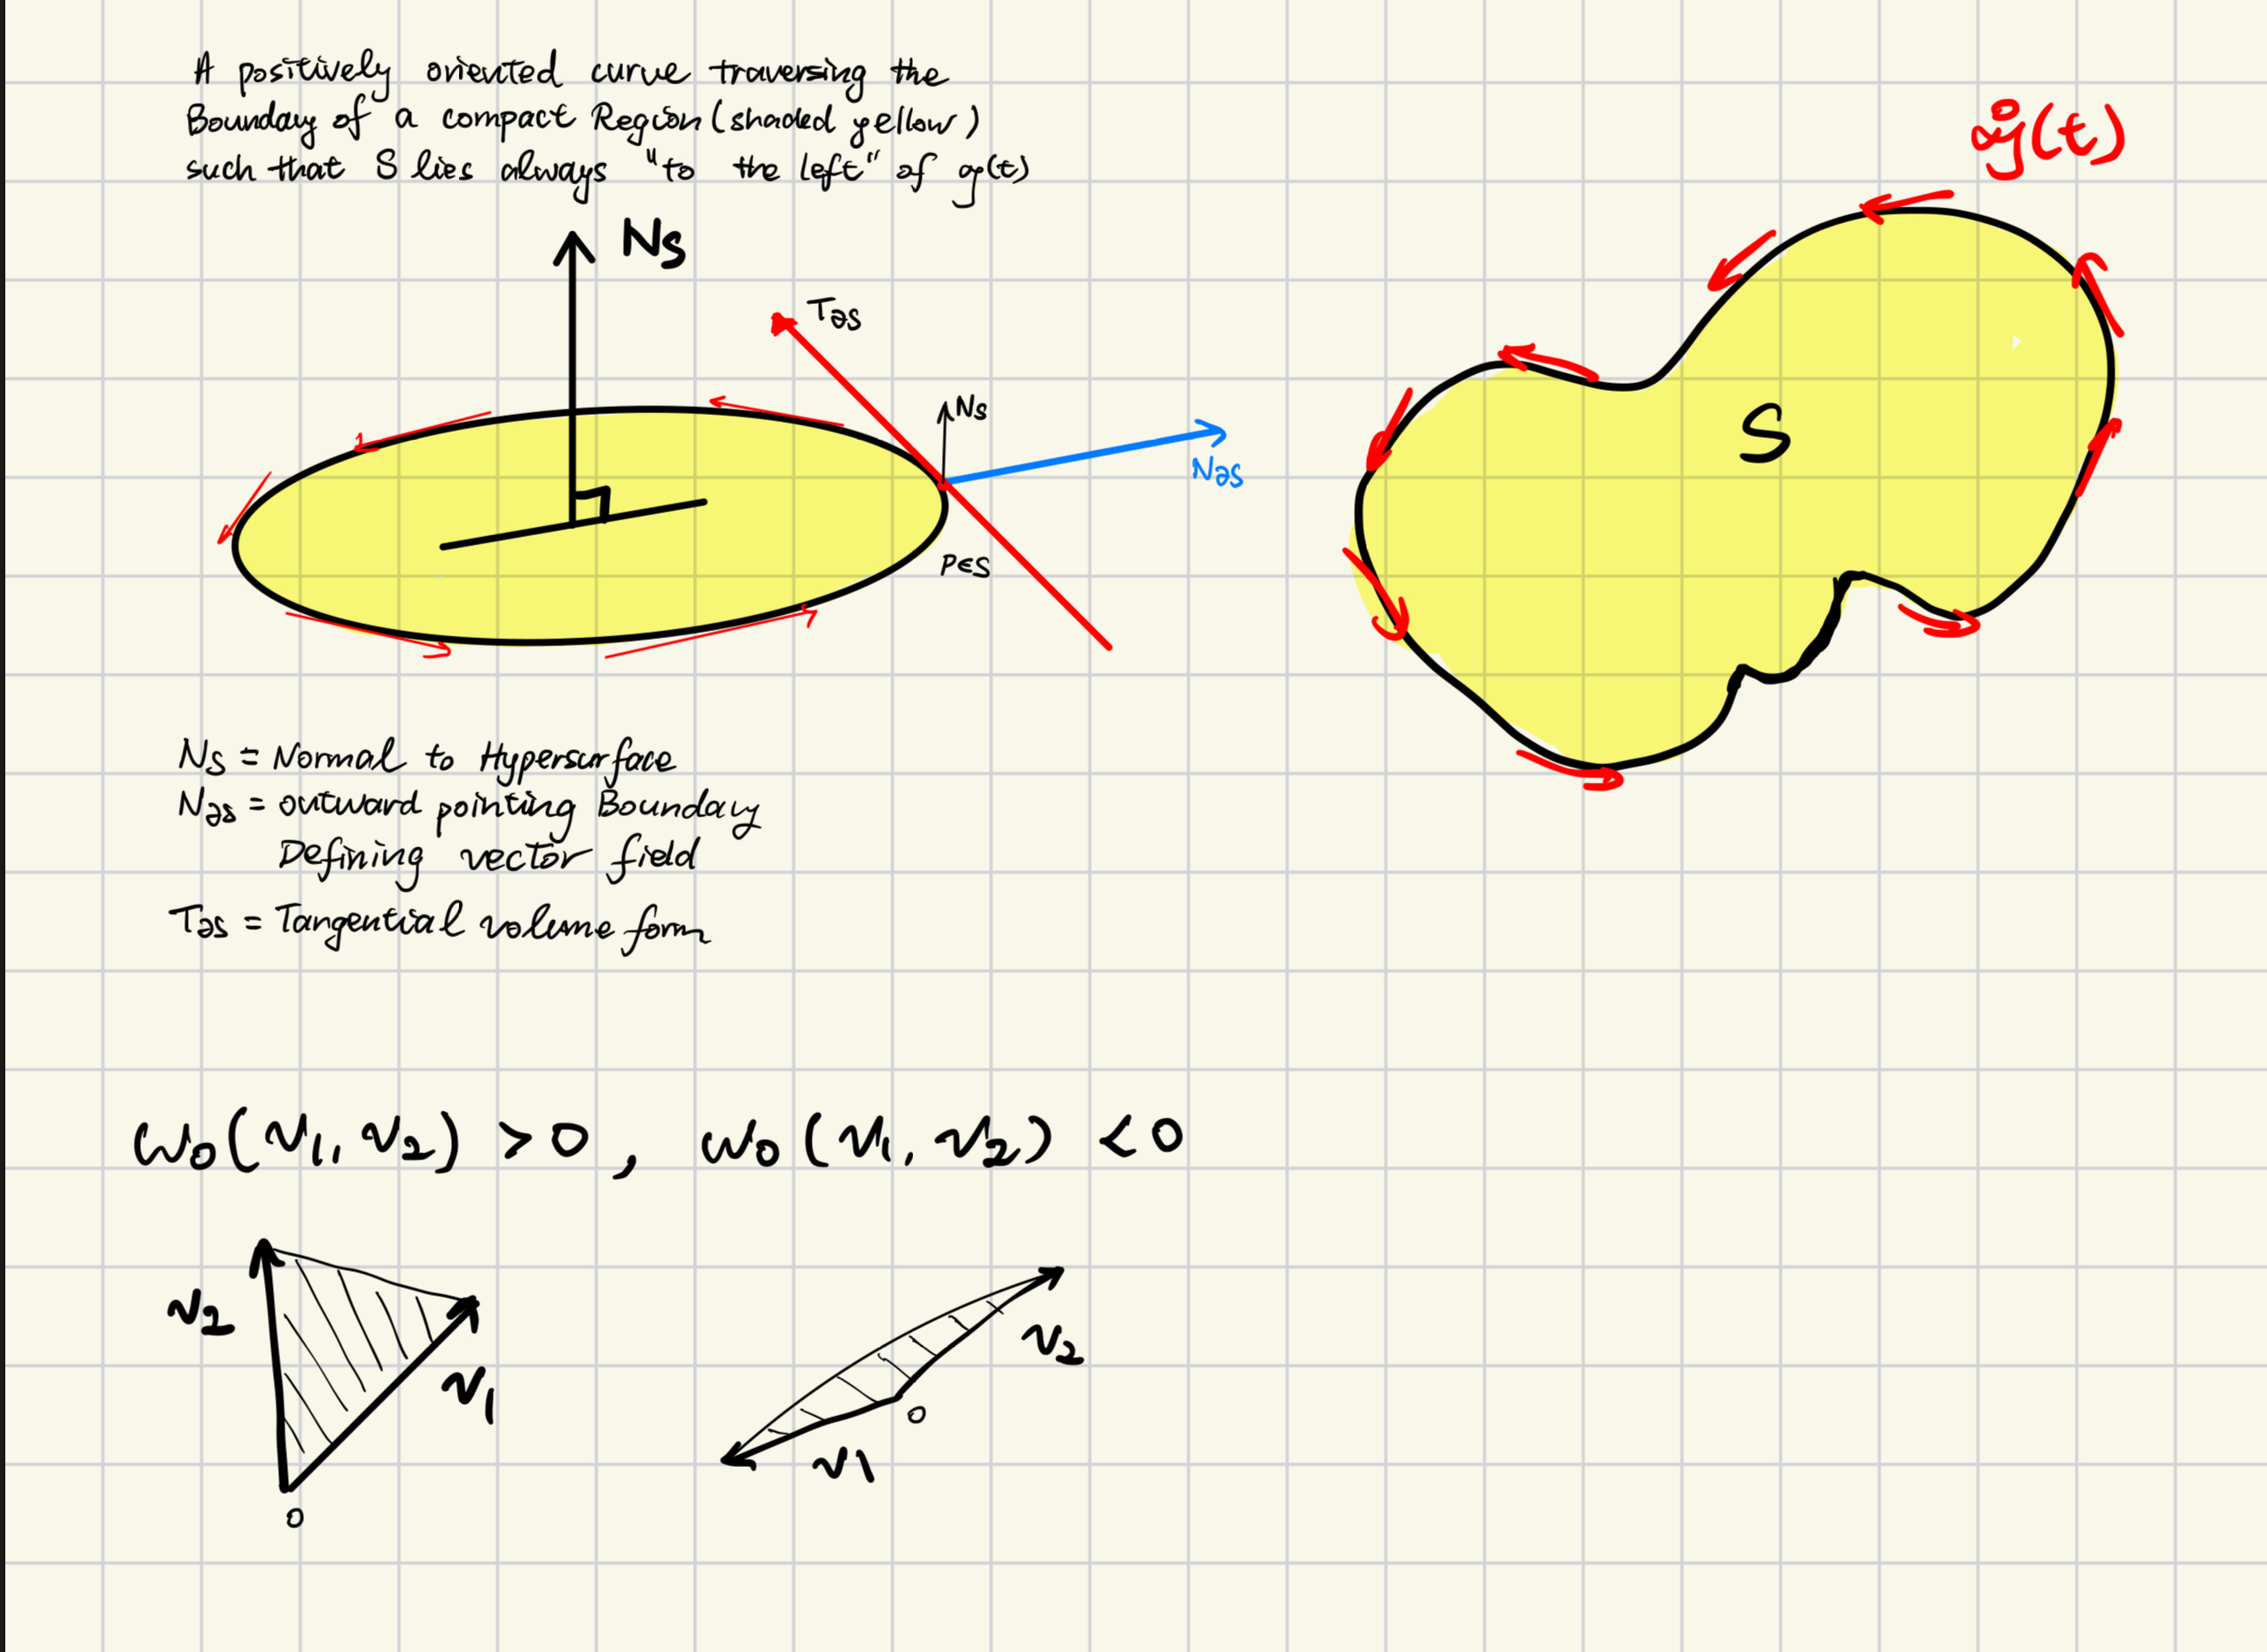
\includegraphics[width=0.5\linewidth]{images/positive-area-opens-to-left-sketch.png}
    \caption{Illustrations of area sign conventions}
    \label{fig:area sign conventions}
\end{figure}
\begin{remark}[Gradient Flow]\label{rmk:gradient flow}
Let $H\in C^\infty(\realtn)$, the \emph{gradient flow} of $H$ is the vector field $\grad H$ such that at every point $p\in \realtn$, and $v_p\in T_p \realtn$:
\begin{quote}
    The \textbf{angle between $\grad{H}(p)$ and $v_p$ is equal to $DH(p)(v_p)$}, where
    \begin{equation}
    H(p+v_p) = H(p) + DH(p)(v_p) + o(\abs{v_p})\quad\text{for sufficiently small }v.
    \label{eq:Frechet Derivative as best possible linear approximation}
\end{equation}
\end{quote}
By the 'angle' we refer to the Euclidean inner product which takes on values in $\real$ instead of in $[-\pi, +\pi]$.
\end{remark}
\begin{definition}[Hamiltonian Flow]
    The \emph{Hamiltonian flow} of $H$ is the vector field $X_H$ such that at every point $p\in \realtn$, and $v_p\in T_p\realtn$:
    \begin{quote}
        The \textbf{symplectic area from $X_H(p)$ to $v_p$ is equal to $DH(p)(v_p)$.}
    \end{quote}
    More precisely, the Hamiltonian flow of $H$ is defined by the sharpening the covector field of $H$:  $X_H = \omega_0^{\wedge}(dH)$, such that
    \begin{equation}
        \omega_0(X_H(p), v_p) = dH(p)(v_p)\quad\text{for all }p\in \realtn,\: v_p\in T_p\realtn.
        \label{eq:hamiltonian flow definition symplectic pairing}
    \end{equation}
\end{definition}
In Euclidean coordinates, the $X_H$ has a simple structure. It can be easily shown that
\[X_H = J\nabla H.\]
\begin{definition}[Regular Hypersurface]\label{def:regular hypersurface}
    A \emph{regular hypersurface} on a smooth manifold $M$ is a subset $S = f^{-1}(c)$ where $f\in C^\infty(M,\real)$, and $df(p)\neq 0$ for every $p\in S$. We call $f$ the \emph{defining function} of $S$ which admits a natural manifold structure that makes $S$ a submanifold of $M$. 
\end{definition}
\begin{wts}[WC Reduction 1 --- Independence of Hamiltonian]
    Let $S$ be a compact, regular hypersurface on $\realtn$.
\end{wts}
\begin{remark}
    By manifold we always mean a $\real$-manifold of class $C^\infty$, modelled over $\realn$ where $n\geq 1$.
\end{remark}
%% Footnote: a differential form is said to be closed whenever its exterior derivative is zero.
%% Footnote: a differential form is said to be exact whenever it is the exterior derivative of another differential form.
%% Poincare's Lemma: if M is a star-shaped domain, then a differential 1-form is closed if and only if it is exact.
%% Fact: Exact forms are always closed, but closed forms are not always exact - depends on deRham cohomology.
%
%
%
\topheader{Symplectic Manifold}
Let $n\geq 1$ be an integer, a \emph{symplectic manifold} of class $C^\infty$ is a real manifold of dimension $2n$ that is equipped with a $2$-form $\omega\in \Omega^2(M)$ such that
\begin{itemize}
    \item $\omega$ is non-degenerate, that is: at every $x\in M$ for every tangent vector $v_1\in T_xM$ there exists another tangent vector $v_2\in T_xM$ such that $\omega(v_1,v_2)$. Alternatively, the flat map is non-singular --- meaning
    \[
        \breve{\omega}(v_1) = \omega(v_1,\cdot) \neq 0\in T^*_xM\quad\forall v_1\in T_xM
    \]
    \item $\omega$ is closed, meaning $d\omega=0$ where $d$ refers to the exterior derivative of $\omega$.
\end{itemize}
We call a $2$-form that satisfies the two properties above a \emph{symplectic form} on $M$. 
\begin{remark}
    All finite-dimensional manifolds hereinafter will be assumed $C^\infty$.
\end{remark}

\topheader{Symplectic Action}
Let us assume $n=1$, and we will be working in $\real^{2}$. We define the \emph{standard symplectic form} represented by the matrix in \cref{eq:std symplectic form r2}


Next, let $x,y\in C^\infty(S^1,\real^{2})$. We define the $a(x,y)$ to be normalized the pointwise integral of \cref{eq:std symplectic action pw r2} but with $\dot{x}$ instead of $x$.
\begin{equation}
    a(x,y) = 2^{-1}\int_{S^1}\omega(\dot{x},y)= 2^{-1}\int_{S^1}\det(\dot{x},y)
    \label{std:std symplectic action loop r2}
\end{equation}
We see that \cref{std:std symplectic action loop r2} computes the area of the triangle being swept by $\dot{x}$ and $y$. We also have the following bound
\[
    2^{-1}\int_{S_1}\abs{\omega(\dot{x},y)}\leq 2^{-1}(\norm{y_1\dot{x}_2}_{L^2} + \norm{y_2\dot{x}_1}_{L^2})
\]

%%
%
%
%
%
We write the general case for $n\geq 1$ as a placeholder. There are two conventions for the matrix $J$. The first one is given in \cref{eq:std symplectic form r2n 1}
\begin{equation}
    J = \begin{bmatrix}
        \dmat{\symatrix,\ddots,\ddots,\symatrix}
    \end{bmatrix}
    \label{eq:std symplectic form r2n 1}
\end{equation}
The second one, given in \cref{eq:std symplectic form r2n 2} is the one we will use.
\begin{equation}
    J =\begin{bmatrix}
        \admat[0]{I_n,-I_n}
    \end{bmatrix}
    \label{eq:std symplectic form r2n 2}
\end{equation}
%
%
%
For a general vector $x\in\realtn$, $Jx = (\UL{x}[n+][n],-\UL{x}[n])$, and $x^TJ = (-\UL{x}[n+][n],-\UL{x}[n])$. 
\begin{itemize}
    \item Computing the time-$1$ map of its flow gives
    \[
        e^Jx = \cos(1)x + \sin(1)Jx
    \]
\end{itemize}
\topheader{Hamiltonian Flows}
Given $f\in C^\infty(\realtn)$, we want to describe what actually is the induced Hamiltonian flow $X_f\in \mathfrak{X}(\realtn)$.\\

The symplectic form now becomes the evaluation map, and,
\begin{quote}
    calculating the area spanned between $X_f$ and another vector $v\in \realtn$, is the same as evaluating $df(v)$.
\end{quote}
so, if $v$ 


%% Here we want to explain what happens in coordinates
Computing the symplectic pairing between $X_H$ and a tangent vector $v_p$, we get
\[
\omega_0\qty(X_H(p),v_p) = \sum_{i=\underline{n}} \det\qty(\mqty[X_H^i & v_p^i \\ X_H^{n+i} & v_p^{n+i}])
\]
Writing the standard symplectic matrix in terms of tensor products, 
\[
    J = \mqty[ 0 & -I_n \\ I_n & 0] = [\delta_{(i,n+j)} - \delta_{(n+i,j)}]_{ij}
\]

\[
    \omega_0^{\wedge}(X_H(p)) = \sum_{i=\underline{n}}
\]

\end{document}

